\documentclass[
  12pt,				    % tamanho da fonte
  openright,			% capítulos começam em pág ímpar (insere página vazia caso preciso)
  oneside,			  % para impressão em recto e verso. Oposto a oneside
  a4paper,			  % tamanho do papel. 
  chapter=TITLE,  % títulos de capítulos convertidos em letras maiúsculas
  section=TITLE,  % títulos de seções convertidos em letras maiúsculas
  english,			  % idioma adicional para hifenização
  french,				  % idioma adicional para hifenização
  spanish,			  % idioma adicional para hifenização
  brazil				  % o último idioma é o principal do documento
]{iftex}

% Importa as macros do projeto
%% Macros de dados do documento
\autor{Artur Dias Rodrigues Vicente}
\titulo{Supervisão e controle de nível com lógica Fuzzy: Uma integração baseada em OPC}
\instituicao{Instituto Federal do Espírito Santo}
\campus{Campus Serra}
\curso{ENGENHARIA DE CONTROLE E AUTOMAÇÃO}
\local{Serra -- ES}
\data{2025}


\preambulo {Trabalho de conclusão de curso, apresentado como parte das atividades para obtenção do título de Bacharel em Engenharia de Controle e Automação, do curso de Engenharia de Controle e Automação do Instituto Federal do Espírito Santo.
\vspace{0.5cm}\\ Orientador: Prof. Dr. Daniel Cruz Cavalieri
}

\examinadori{Prof. Dr. Daniel Cruz Cavalieri}{Instituto Federal do Espírito Santo}
{Campus Serra}
\examinadorii{Prof. Me. Rafael Emerick Zape de Oliveira}{Instituto Federal do Espírito Santo}
{Campus Serra}
\examinadoriii{Prof. Dr. Flávio Garcia Pereira}{Instituto Federal do Espírito Santo}
{Campus Serra}

\approvaldate{28}{Agosto}{2025}


% Ficha catalográfica
\fichabiblioteca{
    Dados Internacionais de Catalogação-na-Publicação (CIP) \\
    (Biblioteca Nilo Peçanha do Instituto Federal do Espírito Santo)
}
\fichaautor{Elaborada por XXXXXXXXXXXXXXXXXXXXX – CRB-X/ES - XXX}
\fichatags{
    1. Redes neurais (Computação).  2. Expressão facial – Processamento de dados. 3. Sistemas de reconhecimento de padrões. 4. Processamento de imagens – Técnicas digitais. 5. Percepção de padrões. 6. Engenharia Elétrica. I. XXXXXXXX, XXXXXXXXXX XXXXXXXXXX.  II. Instituto Federal do Espírito Santo. III. Título.
}

\cutter{X999y}
\cdd{000.00}
\selectlanguage{brazil}

% Arial (para usar times-new-roman, comente as três linhas abaixo)
\usepackage{helvet}
\renewcommand{\familydefault}{\sfdefault}
\renewcommand{\ABNTEXchapterfont}{\bfseries}
% Comandos para revisar o texto
\usepackage{easyReview} 


%% Elementos opcionais
\editardedicatoria{\input{pre_textuais/dedicatoria}}
\editaragradecimentos{Agradeço a Deus por me conceder força, sabedoria e perseverança ao longo desta jornada. Sou profundamente grato à minha família pelo apoio incondicional, incentivo e amor, fundamentais para a realização deste trabalho. 

Estendo meus sinceros agradecimentos a todos os professores que me orientaram com conhecimento, paciência e dedicação, contribuindo significativamente para meu crescimento acadêmico e pessoal.

Por fim, reconheço o Instituto Federal do Espírito Santo por proporcionar recursos, oportunidades e um ambiente propício ao aprendizado e desenvolvimento.}
\editarepigrafe{\thispagestyle{empty}

\begin{minipage}{1cm}

\end{minipage}

\vfill

\begin{center}
\begin{minipage}{11cm}
"A ciência pode divertir e fascinar, mas é a engenharia que muda o mundo."
\end{minipage}
\end{center}

\vspace{1.5cm}

\begin{flushright}
(Asimov, 1988)
\end{flushright}}


% Novos comandos
\newcommand{\ie}{\textit{i.e. }}
\newcommand{\eg}{\textit{e.g. }}

\begin{document}

  % --------------------------------------------------- %
  % CAPAS                                               %
  % --------------------------------------------------- %
  % CAPA E FOLHA DE ROSTO
  \capas
  \imprimircapa
  \imprimirfolhaderosto
  % \imprimirfichacatalografica
  % \includepdf[pages=-]{pre_textuais/ficha.pdf}

  % --------------------------------------------------- %
  % ELEMENTOS PRÉ-TEXTUAIS                              %
  % --------------------------------------------------- %
  % APROVAÇÃO, DEDICATÓRIA, AGRADECIMENTOS, EPÍGRAFE
  \pretextual
  \imprimiraprovacao
  % \includepdf[pages=-]{pre_textuais/aprovacao.pdf}
  % \imprimirdedicatoria
  \imprimiragradecimentos
  \imprimirepigrafe
  
  % RESUMO - PT/EN
  % RESUMO - PT
\begin{resumo}
  \vspace{-15pt}
  
No âmbito da automação industrial, a integração entre sistemas de controle constitui uma necessidade fundamental para o monitoramento e controle eficiente de processos produtivos. Este trabalho apresenta o desenvolvimento de um sistema de supervisão e controle de nível baseado em lógica Fuzzy, integrado através do protocolo OPC (Open Platform Communications).

A lógica Fuzzy, técnica de inteligência artificial que possibilita o tratamento de incertezas e imprecisões inerentes aos processos industriais, demonstra particular adequação para o controle de plantas de nível. Tais sistemas, amplamente utilizados nas indústrias petroquímica, farmacêutica e de alimentos e bebidas, caracterizam-se por sua natureza não linear e frequentemente multivariável, apresentando desafios significativos para técnicas de controle convencionais.

O objetivo principal deste trabalho consiste na implementação de uma arquitetura de integração entre uma API responsável pelo controle Fuzzy e uma planta de nível simulada, utilizando o protocolo OPC como meio de comunicação. Esta abordagem visa demonstrar a viabilidade da aplicação de técnicas de inteligência artificial em ambientes industriais reais, aproveitando-se da padronização e ampla adoção do protocolo OPC na indústria moderna.


  \textbf{Palavras-chave:} Controle de Nível, Controlador Fuzzy, Lógica Fuzzy, C-Sharp, C\#, Automação Industrial, Python, Blazor, WPF, OPC, OPC UA, IHM, Integração de Sistemas.
\end{resumo}

  \thispagestyle{empty}
\captionsenglish

\begin{resumo}


In the field of industrial automation, the integration between control systems is a fundamental requirement for efficient monitoring and control of production processes. This work presents the development of a level supervision and control system based on Fuzzy logic, integrated through the OPC (Open Platform Communications) protocol.

Fuzzy logic, an artificial intelligence technique that enables the handling of uncertainties and imprecisions inherent to industrial processes, proves particularly suitable for level plant control. Such systems, widely used in the petrochemical, pharmaceutical, and food and beverage industries, are characterized by their nonlinear and often multivariable nature, presenting significant challenges for conventional control techniques.

The main objective of this work is to implement an integration architecture between an API responsible for Fuzzy control and a simulated level plant, using the OPC protocol as the communication medium. This approach aims to demonstrate the feasibility of applying artificial intelligence techniques in real industrial environments, taking advantage of the standardization and widespread adoption of the OPC protocol in modern industry.

 \vspace{0.5cm}
 
 \textbf{Keywords:} Level Control, Fuzzy Controller, Fuzzy Logic, C-Sharp, C\#, Industrial Automation, Python, Blazor, WPF, OPC, OPC UA, HMI, Systems Integration. 
\end{resumo}
\captionsbrazil

  % LISTAS E SUMÁRIO
  \imprimirlistafiguras
  \imprimirlistatabelas
  \imprimirsumario

  % --------------------------------------------------- %
  % ELEMENTOS TEXTUAIS                                  %
  % --------------------------------------------------- %
  \textual
  \graphicspath{{figuras/}}
  \chapter{Introdução}
\label{chap:intro}
%\thispagestyle{plain}
\graphicspath{{./Cap1_introducao/Figures/}}

A quarta revolução industrial, denominada Indústria 4.0, representa um paradigma transformador na manufatura global, caracterizada pela integração sistemática de tecnologias digitais avançadas nos processos produtivos. Este movimento revolucionário fundamenta-se na conectividade entre sistemas físicos e digitais, proporcionando maior eficiência, flexibilidade e sustentabilidade aos processos industriais \cite{Schwab2016}. Neste contexto, a automação industrial emerge como elemento central, demandando investimentos significativos em tecnologias que possibilitem a otimização de processos e a redução de custos operacionais.

Os investimentos em tecnologia para automatização têm experimentado crescimento exponencial nas últimas décadas, impulsionados pela necessidade de competitividade global e pela busca por processos mais eficientes e sustentáveis. Segundo dados da Associação Brasileira de Automação Industrial (ABAI), o mercado brasileiro de automação industrial registrou crescimento consistente, evidenciando a importância estratégica deste setor para o desenvolvimento econômico nacional. Tais investimentos abrangem desde a modernização de equipamentos até a implementação de sistemas de controle avançados, visando à otimização de recursos e ao aumento da produtividade.

A utilização de inteligência artificial na indústria constitui uma das principais tendências da Indústria 4.0, oferecendo soluções inovadoras para desafios complexos de controle e otimização. Técnicas como redes neurais, algoritmos genéticos e lógica Fuzzy têm demonstrado eficácia significativa na resolução de problemas industriais que envolvem incertezas, não linearidades e múltiplas variáveis. A lógica Fuzzy, em particular, destaca-se pela sua capacidade de modelar conhecimento humano especializado e tratar informações imprecisas, características comuns em ambientes industriais reais.

O controle automático representa um dos pilares fundamentais da automação industrial moderna, possibilitando a manutenção de variáveis de processo dentro de faixas operacionais desejadas sem intervenção humana direta. A implementação de sistemas de controle automático resulta em benefícios tangíveis, incluindo maior precisão no controle de processos, redução de variabilidade na qualidade do produto, diminuição de custos operacionais e melhoria nas condições de segurança operacional. Ademais, tais sistemas contribuem para a redução do impacto ambiental através da otimização do uso de recursos naturais e energia.

No contexto específico da automação industrial, o controle de nível assume importância crítica em diversas aplicações, desde o armazenamento de matérias-primas até o processamento final de produtos. Sistemas de controle de nível são essenciais para garantir a continuidade operacional, prevenir perdas de produto por transbordamento, evitar danos a equipamentos por operação em vazio e assegurar a qualidade do produto final. Nas indústrias petroquímica, farmacêutica e de alimentos e bebidas, o controle preciso de nível em tanques e reatores é fundamental para manter as condições ideais de processo e atender aos rigorosos padrões de qualidade e segurança exigidos por essas indústrias.

Diante deste cenário, o presente trabalho propõe uma abordagem para o controle de nível industrial, integrando a lógica Fuzzy com o protocolo OPC, visando demonstrar a viabilidade da aplicação de técnicas de inteligência artificial em ambientes industriais reais através de uma arquitetura de integração padronizada e amplamente adotada pela indústria.

\section{Revisão Bibliográfica}
\label{sec:revbibli}

\subsection{Importância do controle de nível}
\label{sec:importancenivel}
O controle de nível em processos industriais constitui uma das variáveis mais críticas para o funcionamento seguro e eficiente de plantas produtivas. A relevância deste tipo de controle é evidenciada em diversos setores industriais, desde aplicações didáticas até implementações em larga escala industrial.

\cite{bacovis2016} realizaram um estudo comparativo entre controladores Fuzzy e PID aplicados em uma planta didática de nível de líquido, demonstrando que o controle adequado de nível é fundamental para o aprendizado e compreensão dos princípios de automação industrial. O trabalho evidencia que plantas de nível são amplamente utilizadas em ambientes educacionais devido à sua capacidade de representar fielmente os desafios encontrados em processos industriais reais, incluindo não linearidades, tempo morto e distúrbios externos.

Na indústria de alimentos e bebidas, \cite{gomes2022} investigou a aplicação da lógica Fuzzy no controle de qualidade na produção de cerveja, onde o controle preciso de nível em tanques de fermentação e maturação é crucial para garantir a qualidade do produto final. O autor demonstra que variações não controladas no nível podem afetar diretamente características organolépticas da cerveja, como aroma, sabor e teor alcoólico, evidenciando a importância crítica do controle de nível em processos biotecnológicos.

Em aplicações de saneamento e abastecimento público, \cite{silveira2021} apresentaram um estudo sobre a aplicação da lógica Fuzzy no controle de nível de reservatório de abastecimento de água, destacando que o controle eficiente de nível é essencial para garantir o fornecimento contínuo e adequado de água potável. Os autores enfatizam que falhas em sistemas de controle de nível podem resultar em desabastecimento populacional, desperdício de recursos hídricos e comprometimento da qualidade da água distribuída.

A importância do controle de nível transcende aspectos puramente técnicos, envolvendo questões econômicas, ambientais e de segurança. Sistemas de controle de nível inadequados podem resultar em perdas significativas de produto, consumo excessivo de energia, riscos ambientais por vazamentos e comprometimento da segurança operacional. Ademais, o controle preciso de nível é fundamental para otimizar o uso de recursos naturais e contribuir para a sustentabilidade de processos industriais.

\subsection{Utilização do OPC em plantas industriais}
\label{sec:utilizacaoopc}
O protocolo OPC (Open Platform Communications) e sua evolução para OPC UA (Unified Architecture) têm revolucionado a comunicação industrial, oferecendo soluções padronizadas para a integração de sistemas heterogêneos em ambientes produtivos. A aplicação desta tecnologia em plantas industriais demonstra sua versatilidade e eficácia na resolução de desafios complexos de interoperabilidade e digitalização.

\cite{carvalho2023} investigaram a digitalização de uma planta industrial utilizando o protocolo de comunicação OPC-UA, focando no sistema educacional CP Lab da Festo. O estudo demonstra como a Indústria 4.0 está impulsionando transformações profundas na indústria através de soluções que aprimoram a produção e elevam a qualidade dos produtos. Os autores evidenciam que tecnologias como IoT, sistemas ciberfísicos, Big Data e computação em nuvem estão remodelando as operações empresariais através da integração de sistemas, criação de fábricas inteligentes e melhoria da eficiência. A pesquisa destaca que a utilização do protocolo OPC UA para conectar módulos ciberfísicos e dispositivos à nuvem possibilita análise de dados em tempo real para identificar status atual, problemas potenciais e tomar decisões mais eficazes.

Em aplicações de manufatura flexível, \cite{silva2023} desenvolveu um sistema de instrumentação para uma planta de manufatura flexível utilizando o padrão OPC-UA embarcado no microcontrolador ESP32. O trabalho evidencia que o OPC-UA é um padrão de comunicação industrial que permite transferência de dados segura e confiável entre diferentes sistemas e dispositivos em setores industriais. O estudo demonstra a viabilidade de implementar servidores OPC-UA em dispositivos embarcados de baixo custo, estabelecendo comunicação entre servidores OPC-UA utilizando a ferramenta Node-RED para transferir dados do sistema de medição para controladores lógicos programáveis (CLP) presentes na planta industrial.

\cite{petrocchi2024} apresentou uma implementação da integração entre tecnologia RFID e o padrão OPC UA aplicada a um sistema de manufatura flexível no laboratório da UNESP campus Sorocaba. O trabalho demonstra que o padrão OPC UA fornece uma troca segura de informações e dados na área da automação industrial, utilizando um protocolo padrão extensível que pode ser empregado em multiplataformas. A pesquisa evidencia que é possível realizar alterações das informações através do sistema de servidor e cliente graças às funcionalidades de acesso aos dados do OPC UA. O desenvolvimento utilizou o ambiente Node-RED para configuração automática do leitor RFID e criação do servidor OPC UA, permitindo leitura e escrita de dados tanto pelo servidor quanto pela interface gráfica.

\cite{souza2024} conduziu um estudo de caso sobre controle e supervisão de processos utilizando o padrão OPC, focando na superação dos desafios de integração entre equipamentos e softwares de diferentes fabricantes devido a protocolos proprietários. O trabalho utilizou o CLP Codesys e o ambiente simulado do Factory IO, com foco na planta industrial Sorting Station, demonstrando como o padrão OPC UA promove a troca de dados e comandos entre sistemas distintos. A pesquisa explora as possibilidades tecnológicas oferecidas por essa integração, evidenciando a capacidade do OPC UA em conectar e comunicar softwares e dispositivos de diferentes fabricantes.

A utilização do OPC em plantas industriais transcende aspectos puramente técnicos, representando um facilitador fundamental para a implementação da Indústria 4.0. Os trabalhos analisados demonstram que a adoção do protocolo OPC UA resulta em maior flexibilidade operacional, redução de custos de integração, melhoria na interoperabilidade entre sistemas e facilita a migração para arquiteturas mais modernas. Ademais, a capacidade do OPC UA de operar em dispositivos embarcados de baixo custo democratiza o acesso a tecnologias avançadas de comunicação industrial, possibilitando a modernização de plantas existentes com investimentos reduzidos.

\subsection{Controle inteligente e OPC em aplicações industriais}
\label{sec:controleintopc}
A convergência entre técnicas de controle inteligente e protocolos de comunicação padronizados como o OPC representa uma das principais tendências na automação industrial moderna. Esta integração possibilita o desenvolvimento de sistemas de controle mais sofisticados, flexíveis e adaptáveis às demandas crescentes da Indústria 4.0, oferecendo soluções inovadoras para desafios complexos de controle e manutenção industrial.

\cite{oliveira2023} desenvolveu um estudo sobre gerenciamento de nível em reservatório de líquidos utilizando lógica Fuzzy e controle PID, implementando uma arquitetura integrada baseada em OPC para comunicação entre sistemas. O trabalho apresenta um sistema amplamente utilizado nas instalações industriais: o controle de nível de tanque, realizado através do software CodeSys e Matlab/Simulink, com simulação no ambiente Factory I/O. A pesquisa desenvolveu dois controladores distintos: um baseado em lógica Fuzzy e outro em controle PID, utilizando o protocolo de comunicação OPC para estabelecer a comunicação entre o CLP, Matlab e Factory I/O. O autor evidencia que a utilização da ferramenta Fuzzy Logic Designer do Matlab, em conjunto com o Simulink, proporcionou análise detalhada do comportamento do sistema, demonstrando controle satisfatório do sistema simulado de tanque. Esta abordagem integrada ilustra como a combinação de técnicas de controle inteligente com protocolos de comunicação padronizados pode resultar em sistemas de controle mais eficazes e facilmente integráveis a arquiteturas industriais existentes.

\cite{coretti2025} investigou a automação com redes inteligentes para manutenção de sistemas de controle de processos industriais, focando no desenvolvimento de mecanismos para digitalização da malha de controle de vazão e tomada de decisão para análise da manutenção de sistemas automatizados. O trabalho utiliza conceitos da Indústria 4.0 e algoritmos de inteligência artificial para melhorar a visibilidade das malhas de controle fechadas e dos ativos da fábrica. A pesquisa propõe uma abordagem que facilita à equipe industrial de manutenção e operação maior facilidade na gestão dos sistemas de automação e tomada de decisões precisas, sem grandes interrupções do processo produtivo. O autor demonstra que a implementação de redes industriais inteligentes, combinada com manutenção proativa e softwares industriais, permite gestão mais eficiente das fábricas com custos reduzidos. A proposta inclui interface de digitalização da malha de controle livre, configurada em blocos funcionais na web, evidenciando a tendência de integração entre sistemas de automação tradicionais e plataformas digitais modernas.

A integração entre controle inteligente e OPC em aplicações industriais representa uma evolução natural dos sistemas de automação, proporcionando benefícios significativos em termos de flexibilidade, manutenibilidade e capacidade de integração. Os trabalhos analisados demonstram que esta abordagem permite não apenas melhor desempenho de controle através de técnicas inteligentes como lógica Fuzzy, mas também facilita a implementação de estratégias de manutenção preditiva e proativa através da padronização de comunicação proporcionada pelo OPC.

Ademais, a utilização de protocolos OPC em sistemas de controle inteligente contribui para a democratização do acesso a tecnologias avançadas, permitindo que empresas de diferentes portes implementem soluções sofisticadas de automação sem dependência de fornecedores específicos. Esta característica é fundamental para a competitividade industrial no contexto da Indústria 4.0, onde a capacidade de adaptação rápida às mudanças tecnológicas e de mercado constitui vantagem estratégica crítica.

\section{Objetivos}
\label{sec:obj}
Os objetivos deste trabalho podem ser definidos da seguinte forma:

\subsection{Objetivo Geral}
\label{sec:objgeral}
Desenvolver e comparar o desempenho de dois métodos de controle, PID e PID-Fuzzy, em uma planta de controle de luminosidade, a fim de identificar qual método oferece melhor resposta em termos de estabilidade, tempo de resposta e precisão.

\subsection{Objetivos Específicos}
\label{sec:objespec}
Para alcançar o objetivo geral proposto, foram definidos os seguintes objetivos específicos:

\begin{itemize}
\item Caracterização do sistema de controle: Extrair os parâmetros Fuzzy da planta de nível, identificando e definindo as variáveis de entrada e saída do sistema, bem como suas respectivas funções de pertinência e regras de inferência necessárias para o controle eficaz do processo.
\item Desenvolvimento da API de controle: Desenvolver uma API especializada utilizando a linguagem Python, implementando os algoritmos de lógica Fuzzy baseados nos parâmetros previamente definidos, garantindo flexibilidade, robustez e facilidade de integração com sistemas externos.
\item Implementação da aplicação de integração: Desenvolver uma aplicação utilizando a linguagem C-Sharp para promover a integração entre a API de controle Fuzzy e a planta de nível, implementando os protocolos de comunicação OPC necessários para estabelecer a troca de dados em tempo real entre os sistemas.
\item Desenvolvimento da interface humano-máquina: Criar uma IHM (Interface Humano-Máquina) intuitiva e funcional que permita a configuração dinâmica da API e do cliente OPC, bem como a visualização em tempo real do controle de nível, proporcionando monitoramento eficiente e facilidade de operação do sistema integrado.
\item Análise de desempenho: Analisar os resultados obtidos através de testes e simulações, avaliando parâmetros como estabilidade do controle, tempo de resposta, precisão no seguimento de referência, robustez a distúrbios e eficácia da comunicação OPC, documentando as conclusões e contribuições do trabalho para a área de automação industrial.
\end{itemize}

\section{Estrutura do Texto}
Este trabalho está organizado em seis capítulos, estruturados de forma a apresentar uma sequência lógica e progressiva do desenvolvimento da pesquisa, desde a fundamentação teórica até a análise dos resultados obtidos.

\begin{itemize}
\item Capítulo 1 - Introdução: Apresenta o contexto geral da pesquisa, abordando a importância do controle de nível em plantas industriais, a utilização do protocolo OPC em ambientes produtivos e a convergência entre controle inteligente e comunicação OPC. Este capítulo também define os objetivos do trabalho e estabelece a justificativa para a integração de técnicas de lógica Fuzzy com protocolos de comunicação padronizados.
\item Capítulo 2 - Fundamentação Teórica: Explora a evolução histórica dos sistemas de controle, desde as técnicas clássicas até as abordagens modernas, destacando onde o controle Fuzzy se posiciona nesta evolução tecnológica. Adicionalmente, examina a utilização de protocolos de comunicação em plantas industriais, enfatizando a importância da padronização e interoperabilidade para a Indústria 4.0.
\item Capítulo 3 - Metodologia: Detalha a metodologia empregada no desenvolvimento do trabalho, incluindo a justificativa para a escolha da planta de nível como objeto de estudo, a seleção da tecnologia Python para criação da API de controle Fuzzy, e a definição da tecnologia para desenvolvimento da Interface Humano-Máquina (IHM), fundamentando cada decisão tecnológica com base em critérios técnicos e práticos.
\item Capítulo 4 - Desenvolvimento: Apresenta o processo de desenvolvimento dos componentes principais do sistema integrado, incluindo a implementação da API de controle Fuzzy, o desenvolvimento da IHM para monitoramento e configuração, e a criação do cliente OPC UA para estabelecer a comunicação entre os diferentes módulos do sistema.
\item Capítulo 5 - Resultados e Discussão: Analisa os resultados obtidos através da integração entre a API de controle Fuzzy e a planta de nível via protocolo OPC, apresentando métricas de desempenho, estabilidade do sistema e eficácia da comunicação, bem como a discussão crítica dos resultados em relação aos objetivos propostos.
\item Capítulo 6 - Conclusões e Trabalhos Futuros: Sintetiza as principais conclusões do trabalho, destacando as contribuições para a área de automação industrial e controle inteligente, além de propor direcionamentos para trabalhos futuros que possam ampliar e aprofundar os resultados obtidos nesta pesquisa.
\end{itemize}
  \chapter{Fundamentação Teórica}
\label{cap:rev.teorica}
%\thispagestyle{plain}
\graphicspath{{./Cap2_Revisao_Teorica/Figures/}}

A evolução dos sistemas de controle automático reflete o desenvolvimento tecnológico da humanidade, desde os primeiros mecanismos de realimentação até os modernos sistemas baseados em inteligência artificial. Os primórdios do controle automático remontam aos reguladores mecânicos do século XVIII, como o regulador centrífugo de James Watt para máquinas a vapor, estabelecendo os fundamentos do controle por realimentação. A formalização matemática destes conceitos ocorreu no século XX, com o desenvolvimento da teoria de controle clássico, caracterizada pela utilização de técnicas baseadas em função de transferência e análise no domínio da frequência \cite{ogata2009}.

O controlador PID (Proporcional-Integral-Derivativo) emergiu como a solução mais amplamente adotada no controle clássico, oferecendo simplicidade de implementação e eficácia em uma ampla gama de aplicações industriais. Sua popularidade deve-se à capacidade de fornecer controle estável e responsivo através do ajuste de três parâmetros fundamentais: ganho proporcional, tempo integral e tempo derivativo \cite{villaca2013}.

A década de 1960 marcou o início da era do controle moderno, caracterizada pela representação de sistemas em espaço de estados e pela utilização de métodos de otimização. Esta abordagem permitiu o tratamento de sistemas multivariáveis e não lineares de forma mais sistemática, superando limitações do controle clássico. O controle moderno introduziu conceitos como controlabilidade, observabilidade e estabilidade no sentido de Lyapunov, com técnicas como o regulador linear quadrático (LQR) e o filtro de Kalman proporcionando ferramentas poderosas para o projeto de controladores ótimos \cite{franklin2015}.

O reconhecimento de que os modelos matemáticos são sempre aproximações da realidade levou ao desenvolvimento do controle robusto nas décadas de 1980 e 1990. Esta abordagem considera explicitamente as incertezas do modelo, garantindo estabilidade e desempenho satisfatório mesmo na presença de variações paramétricas e distúrbios não modelados.

A lógica Fuzzy, introduzida por Lotfi Zadeh em 1965, representa uma abordagem fundamentalmente diferente para o controle de sistemas, baseada na capacidade humana de raciocinar com informações imprecisas e tomar decisões em ambientes de incerteza. Esta técnica emerge como uma ponte entre o controle convencional e a inteligência artificial aplicada, posicionando-se como uma alternativa às limitações dos métodos clássicos e modernos \cite{zadeh1965}.

O desenvolvimento do controle Fuzzy surge em resposta às dificuldades encontradas pelos métodos convencionais em lidar com sistemas complexos, não lineares e mal definidos matematicamente. Enquanto o controle clássico e moderno dependem de modelos matemáticos precisos, o controle Fuzzy permite a incorporação de conhecimento heurístico e experiência operacional diretamente no algoritmo de controle, dispensando a necessidade de modelagem matemática rigorosa \cite{mamdani1975}.

O controle Fuzzy posiciona-se na evolução dos sistemas de controle como uma abordagem complementar que preenche lacunas deixadas pelos métodos convencionais. Sua principal contribuição reside na capacidade de tratar incertezas e imprecisões de forma natural, oferecendo robustez e simplicidade de implementação em aplicações onde modelos matemáticos precisos são difíceis de obter ou onde existe conhecimento heurístico valioso disponível \cite{ross2010}.

A integração eficiente de sistemas em ambientes industriais depende fundamentalmente da capacidade de comunicação entre dispositivos heterogêneos. A evolução dos protocolos de comunicação industrial reflete a crescente necessidade de interoperabilidade, segurança e eficiência na troca de informações. A comunicação industrial evoluiu de sistemas proprietários isolados para padrões abertos e interoperáveis, onde inicialmente cada fabricante desenvolvia seus próprios protocolos, resultando em "ilhas de automação" com limitada capacidade de integração \cite{stenerson2015}.

A necessidade de interoperabilidade levou ao desenvolvimento de padrões como Modbus, Profibus e DeviceNet. O OPC (Open Platform Communications) foi desenvolvido para resolver problemas de interoperabilidade em automação industrial, estabelecendo um padrão para comunicação entre aplicações de diferentes fornecedores. Baseado inicialmente na tecnologia DCOM da Microsoft, o OPC Classic proporcionou avanços significativos, mas suas limitações, incluindo dependência de plataforma e problemas de segurança, levaram ao desenvolvimento do OPC UA (Unified Architecture) \cite{mahnke2009}.

\cite{carvalho2023} investigaram a digitalização de uma planta industrial utilizando o protocolo de comunicação OPC-UA, demonstrando como a Indústria 4.0 está impulsionando transformações profundas na indústria através de soluções que aprimoram a produção. A pesquisa destaca que a utilização do protocolo OPC UA para conectar módulos ciberfísicos e dispositivos à nuvem possibilita análise de dados em tempo real para identificar status atual, problemas potenciais e tomar decisões mais eficazes.

\cite{souza2024} conduziu um estudo de caso sobre controle e supervisão de processos utilizando o padrão OPC, focando na superação dos desafios de integração entre equipamentos e softwares de diferentes fabricantes devido a protocolos proprietários. O trabalho utilizou o CLP Codesys e o ambiente simulado do Factory IO, demonstrando como o padrão OPC UA promove a troca de dados e comandos entre sistemas distintos.

O OPC UA representa uma arquitetura completamente nova, projetada para ser independente de plataforma, segura, escalável e orientada a serviços. Utiliza uma arquitetura em camadas que separa a lógica de aplicação dos detalhes de comunicação, com modelo de informação baseado em uma estrutura hierárquica de nós e referências que permite representar informações complexas de forma padronizada e extensível \cite{leitner2006}.

A utilização de protocolos de comunicação padronizados em plantas industriais transcende aspectos puramente técnicos, representando um facilitador fundamental para a implementação da Indústria 4.0. O OPC UA alinha-se perfeitamente com os princípios da Indústria 4.0, facilitando a integração de sistemas ciberfísicos, permitindo comunicação entre sistemas heterogêneos, suportando diversos paradigmas de comunicação e adaptando-se desde dispositivos de campo até sistemas na nuvem \cite{jasperneite2012}.

A combinação de protocolos padronizados como OPC UA com técnicas de controle inteligente, incluindo lógica Fuzzy, oferece oportunidades únicas para a criação de sistemas de automação mais eficientes e adaptáveis. Esta integração permite distribuição de inteligência em diferentes níveis da hierarquia de controle, flexibilidade arquitetural onde mudanças nos algoritmos de controle não afetam a infraestrutura de comunicação, reutilização de componentes e manutenibilidade através da separação clara entre lógica de controle e comunicação.

\cite{oliveira2023} desenvolveu um estudo sobre gerenciamento de nível em reservatório de líquidos utilizando lógica Fuzzy e controle PID, implementando uma arquitetura integrada baseada em OPC para comunicação entre sistemas. O trabalho demonstrou controle satisfatório do sistema simulado de tanque, ilustrando como a combinação de técnicas de controle inteligente com protocolos de comunicação padronizados pode resultar em sistemas de controle mais eficazes e facilmente integráveis.

A convergência entre controle inteligente e comunicação padronizada representa um paradigma fundamental para a automação industrial moderna, proporcionando a base tecnológica necessária para implementar os conceitos da Indústria 4.0 de forma eficaz e sustentável. Esta integração facilita a implementação de estratégias de manutenção preditiva e proativa, contribui para a democratização do acesso a tecnologias avançadas e permite que empresas de diferentes portes implementem soluções sofisticadas de automação sem dependência de fornecedores específicos.


  \chapter{Metodologia}
\label{cap:metodologia}

A arquitetura proposta na Figura \ref{fig:estrutura} fundamenta-se na integração de quatro componentes principais organizados de forma modular para proporcionar uma solução completa para controle de nível industrial distribuída.

\begin{figure}[H]
    \centering
    \caption[Arquitetura do sistema de controle de nível com lógica Fuzzy integrado via OPC UA.]{Arquitetura do sistema de controle de nível com lógica Fuzzy integrado via OPC UA.}
    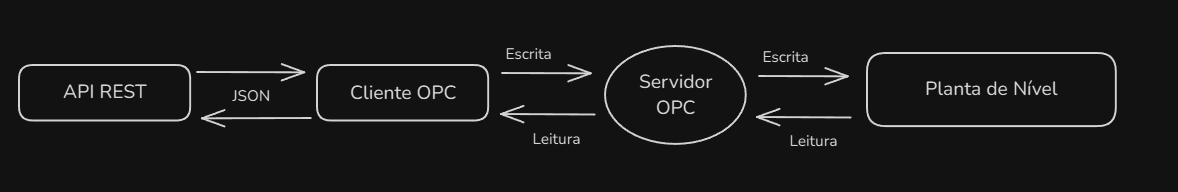
\includegraphics[width=1\textwidth]{figuras/imagens/estrutura.png}
    \label{fig:estrutura}
    \footnotesize Fonte: Dias, 2025. % Ajuste para a fonte
\end{figure}

\begin{itemize}
\item Planta de nível simulada (Matlab/Simulink): Elemento central do sistema representando o processo industrial a ser controlado. Desenvolvida no ambiente Matlab/Simulink.
\item API REST de controle Fuzzy: Núcleo inteligente responsável pela implementação dos algoritmos de controle baseados em lógica Fuzzy.
\item Cliente OPC UA integrado com IHM: Componente intermediário que estabelece comunicação segura via protocolo OPC UA. Responsável pela leitura periódica das variáveis de processo, consumo da API de controle Fuzzy através de requisições HTTP e escrita dos sinais de controle. Integra uma IHM intuitiva para visualização em tempo real, monitoramento, configuração e intervenção manual.
\item Desenvolvimento da interface humano-máquina: Criar uma IHM (Interface Humano-Máquina) intuitiva e funcional que permita a configuração dinâmica da API e do cliente OPC, bem como a visualização em tempo real do controle de nível, proporcionando monitoramento eficiente e facilidade de operação do sistema integrado.
\item Servidor OPC: Ponte de comunicação que expõe as variáveis da planta simulada no espaço de endereçamento OPC. Disponibiliza variáveis garantindo interoperabilidade, segurança e escalabilidade.
\end{itemize}

\section{Escolha da planta de nível}
\label{sec:escolhaplanta}

Para o presente trabalho foi selecionada a planta de nível de água em tanque disponível como exemplo no conjunto de bibliotecas do Matlab, especificamente o modelo `sltank`. Esta escolha justifica-se pelo fato de que a proposta do trabalho é o desenvolvimento da integração entre sistemas e não a parametrização de uma nova planta de nível, além de permitir validação com uma referência estabelecida na literatura técnica.

O sistema de controle de nível de água em tanque apresenta características não lineares típicas de processos industriais reais. O controle é realizado através de uma válvula que regula o fluxo de entrada de água no tanque, enquanto a vazão de saída depende do diâmetro do tubo de saída (constante) e da pressão no tanque, que varia proporcionalmente ao nível de água. Esta característica confere ao sistema comportamento dinâmico não linear, tornando-o adequado para demonstrar as vantagens da aplicação de técnicas de controle inteligente.

O sistema de controle de nível apresenta as seguintes variáveis principais:

Variáveis de entrada do controlador Fuzzy:

\begin{itemize}
\item level (erro de nível): Diferença entre o nível desejado (setpoint) e o nível atual de água no tanque, medida em unidades de altura. Esta variável representa o desvio que o sistema deve corrigir para manter o nível na referência estabelecida.
\item rate (taxa de variação do nível): Derivada temporal do nível de água, indicando a velocidade de variação do nível no tanque. Esta variável fornece informação sobre a tendência de comportamento do sistema, permitindo ações antecipativas do controlador.
\end{itemize}

Variável de saída do controlador Fuzzy:

\begin{itemize}
\item valve (sinal de controle da válvula): Taxa de abertura ou fechamento da válvula de controle de entrada, expressa em percentual ou unidades normalizadas. Este sinal determina a vazão de entrada de água no tanque, constituindo a ação de controle aplicada ao processo.
\end{itemize}

A representação da planta está definida conforme a Figura \ref{fig:planta}.

\begin{figure}[H]
    \centering
    \caption[Planta de nível de água em tanque do Matlab/Simulink (modelo sltank).]{Planta de nível de água em tanque do Matlab/Simulink (modelo sltank).}
    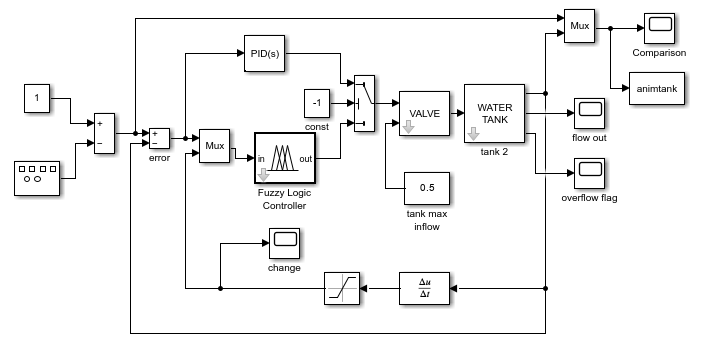
\includegraphics[width=1\textwidth]{figuras/imagens/plantamatlab.png}    
    {Fonte: Dias, 2025.}
    \label{fig:planta}
\end{figure}

\section{API de controle Fuzzy}
\label{sec:apifuzzy}

A implementação da API de controle Fuzzy constitui o núcleo inteligente do sistema proposto, responsável pela execução dos algoritmos de lógica Fuzzy que determinam as ações de controle aplicadas à planta de nível. A escolha da linguagem Python para o desenvolvimento desta API justifica-se por sua ampla disponibilidade de bibliotecas especializadas em sistemas Fuzzy, facilidade de desenvolvimento de APIs REST e capacidade de integração com diferentes tecnologias.

A API segue o padrão arquitetural REST (Representational State Transfer), proporcionando interface padronizada para integração com a IHM. Esta abordagem garante flexibilidade na comunicação, permitindo que diferentes clientes possam consumir os serviços de controle independentemente da plataforma ou tecnologia utilizada. A estrutura modular permite separação clara entre a lógica de controle Fuzzy e a interface de comunicação, facilitando manutenção e futuras expansões do sistema.

O controlador Fuzzy utiliza a parametrização extraída da planta de nível do Matlab (modelo `sltank`), adaptada para implementação em Python. Esta escolha metodológica assegura compatibilidade com a literatura técnica existente e permite validação dos resultados através de comparação com implementações de referência. A API implementa duas variáveis de entrada (erro de nível e taxa de variação) e uma variável de saída (sinal de controle da válvula), utilizando funções de pertinência triangulares e trapezoidais com universos de discurso normalizados.

A base de regras implementada contempla 49 regras de inferência (matriz 7x7), desenvolvidas com base no conhecimento heurístico sobre comportamento de sistemas de controle de nível. A estratégia de controle privilegia ação corretiva proporcional ao erro, comportamento antecipativo baseado na taxa de variação e estabilização para pequenos desvios.

\section{Desenvolvimento da IHM}
\label{sec:devihm}

O desenvolvimento da Interface Humano-Máquina (Figura 3) constitui o componente de interação e supervisão do sistema integrado, proporcionando visualização em tempo real, monitoramento das variáveis de processo e capacidade de intervenção manual no sistema de controle. A escolha da linguagem C-Sharp para o desenvolvimento da IHM justifica-se por sua robustez na criação de aplicações desktop, ampla disponibilidade de bibliotecas para comunicação OPC UA e facilidade de integração com APIs REST.

A representação da IHM está definida conforme a Figura \ref{fig:ihm}.

\begin{figure}[H]
    \centering
    \caption[Interface Humano-Máquina desenvolvida em C\# para supervisão e controle.]{Interface Humano-Máquina desenvolvida em C\# para supervisão e controle.}
    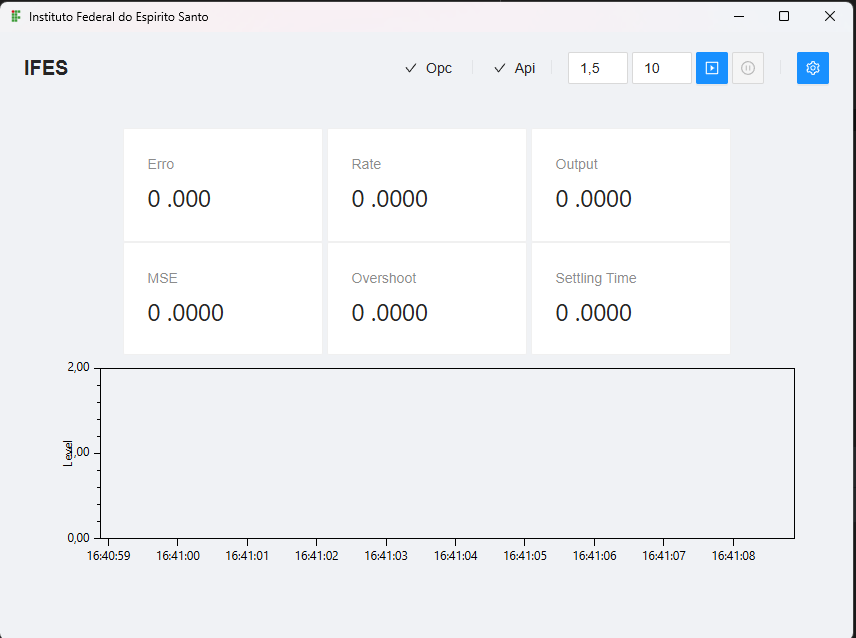
\includegraphics[width=1\textwidth]{figuras/imagens/ihm.png}    
    {Fonte: Dias, 2025.}
    \label{fig:ihm}
\end{figure}

A IHM segue uma arquitetura cliente-servidor, atuando simultaneamente como cliente OPC UA para comunicação com a planta simulada e cliente HTTP para consumo da API de controle Fuzzy. Esta abordagem dual permite que a aplicação funcione como elemento centralizador da arquitetura, coordenando o fluxo de dados entre todos os componentes do sistema. A estrutura modular facilita a manutenção e permite expansões futuras sem comprometer a funcionalidade existente.

A aplicação implementa comunicação bidirecional com o servidor OPC UA, realizando leitura periódica das variáveis de processo (nível atual, setpoint e sinais de controle) e escrita dos comandos de controle calculados pela API Fuzzy. Esta integração utiliza bibliotecas especializadas em OPC UA para C-Sharp, garantindo conformidade com os padrões industriais e compatibilidade com diferentes servidores OPC. A configuração das tags OPC é realizada de forma dinâmica, permitindo adaptação a diferentes configurações de planta sem necessidade de recompilação.

A interface gráfica proporciona visualização intuitiva das variáveis de processo através de gráficos em tempo real, indicadores visuais de status e controles para configuração de parâmetros operacionais. A aplicação implementa funcionalidades de monitoramento contínuo, registro de dados históricos e alarmes para condições de operação anômalas. A integração com a API de controle Fuzzy é realizada através de requisições HTTP periódicas, enviando as variáveis de processo e recebendo os sinais de controle calculados, garantindo operação em tempo real adequada para aplicações de controle industrial.

\section{Integração e Testes}
\label{sec:intetestes}

A metodologia de integração e testes constitui a fase de validação do sistema integrado, responsável por verificar a eficácia da arquitetura proposta através da avaliação do desempenho do controle Fuzzy distribuído via protocolo OPC UA. Esta etapa metodológica visa demonstrar a viabilidade da integração entre sistemas heterogêneos mantendo ou superando o desempenho de controle obtido com implementações convencionais.

A estratégia de integração segue uma abordagem incremental, iniciando com testes unitários de cada componente individual, progredindo para testes de integração entre pares de componentes e culminando com a validação do sistema completo. Esta metodologia garante identificação precoce de problemas de compatibilidade e permite refinamento progressivo da arquitetura antes dos testes finais de desempenho.

\begin{itemize}
\item Testes de componentes individuais: Validação isolada da API de controle Fuzzy, verificação da funcionalidade da IHM, teste de comunicação OPC UA entre servidor e cliente, e confirmação da estabilidade da planta simulada. Esta fase assegura que cada elemento funcione corretamente antes da integração.
\item Testes de integração por pares: Verificação da comunicação entre IHM e API Fuzzy via HTTP, validação da troca de dados entre IHM e servidor OPC UA, e teste da sincronização temporal entre os componentes. Esta etapa identifica problemas de interface e protocolo de comunicação.
\item Testes de sistema completo: Avaliação do desempenho de controle com todos os componentes integrados, medição de latências de comunicação, verificação da robustez do sistema a falhas temporárias de comunicação, e análise da estabilidade em operação contínua prolongada.
\end{itemize}

A metodologia de avaliação de desempenho baseia-se na comparação entre duas configurações de controle: o sistema integrado proposto (API Fuzzy distribuída via OPC UA) e o sistema de referência (controlador Fuzzy nativo do Matlab aplicado diretamente à planta). Esta abordagem comparativa permite quantificar o impacto da arquitetura distribuída no desempenho de controle.

Critérios de avaliação estabelecidos:

\begin{itemize}
\item Estabilidade: Capacidade do sistema de manter controle estável sem oscilações persistentes.
\item Tempo de acomodação: intervalo necessário para que a resposta do sistema atinja e permaneça dentro de 2\% do valor final.
\item Precisão em regime permanente: Desvio percentual entre o valor desejado e o valor alcançado em estado estacionário.
\item Latência de comunicação: Tempo de resposta da arquitetura distribuída comparado ao sistema centralizado.
\end{itemize}

  \chapter{Desenvolvimento}
\label{cap:desenvolvimento}

Este capítulo apresenta a implementação prática dos componentes definidos na metodologia, detalhando o desenvolvimento da API de controle Fuzzy, da Interface Humano-Máquina (IHM) e da integração via protocolo OPC UA. O desenvolvimento seguiu uma abordagem modular, onde cada componente foi implementado e testado individualmente antes da integração final, garantindo funcionalidade e robustez do sistema completo.

A implementação baseia-se na arquitetura distribuída proposta, onde a API de controle Fuzzy desenvolvida em Python atua como núcleo inteligente, a IHM em C\# proporciona interface de supervisão e controle, e a comunicação OPC UA garante interoperabilidade e padronização na troca de dados. Esta estrutura modular facilita manutenção, permite expansões futuras e assegura conformidade com padrões industriais estabelecidos.

\section{Protocolo de comunicação OPC}
\label{sec:opc}

O protocolo OPC UA (OPC Unified Architecture) constitui a base fundamental de comunicação da arquitetura proposta, proporcionando interoperabilidade e padronização na troca de dados entre a planta de nível simulada e a IHM. O OPC (Open Platform Communications) representa um conjunto de especificações padronizadas que definem a interface entre clientes e servidores em sistemas de automação industrial, facilitando a comunicação entre dispositivos de hardware e software de diferentes fornecedores \cite{opc2025a}.

O desenvolvimento do OPC UA surge como evolução natural do OPC Classic, criado para superar limitações fundamentais dos protocolos proprietários que resultavam em "ilhas de automação" isoladas. O OPC UA fundamenta-se em uma arquitetura orientada a serviços que separa claramente a funcionalidade de aplicação dos detalhes específicos da tecnologia de comunicação subjacente, proporcionando flexibilidade excepcional e operação independente de plataforma, sistema operacional ou tecnologia de rede utilizada \cite{opc2025b}.

A arquitetura OPC UA estrutura-se em múltiplas camadas funcionais que garantem robustez e versatilidade na comunicação industrial. A \textbf{camada de transporte} suporta múltiplos protocolos de comunicação incluindo TCP/IP binário nativo, HTTPS e WebSockets, permitindo implementação desde dispositivos embarcados até aplicações em nuvem. A \textbf{camada de serialização} oferece codificação binária otimizada para eficiência máxima e codificação JSON/XML para facilitar integração web e interoperabilidade ampliada \cite{opc2025b}.

O \textbf{modelo de informação orientado a objetos} constitui o núcleo conceitual inovador do OPC UA, definindo estruturação hierárquica de dados através de espaço de endereçamento baseado em nós interconectados por referências tipificadas. Este modelo permite representação rica e semântica de informações industriais, suportando desde variáveis simples até modelos complexos de equipamentos e processos. Os tipos fundamentais incluem \textbf{Object Nodes} para entidades físicas ou lógicas, \textbf{Variable Nodes} para dados de processo, \textbf{Method Nodes} para operações remotas e \textbf{DataType Nodes} para definições estruturadas \cite{opc2025b}.

O protocolo implementa paradigma cliente-servidor robusto onde servidores OPC UA expõem funcionalidades através de espaços de endereçamento estruturados, enquanto clientes acessam informações mediante serviços padronizados. O processo de estabelecimento de conexão segue rigorosamente especificações IEC 62541, iniciando com \textbf{descoberta automática de endpoints}, seguida por \textbf{estabelecimento de canal seguro} com negociação de políticas de segurança e \textbf{criação de sessão autenticada} com controle de acesso baseado em certificados.

A estratégia de comunicação baseia-se em \textbf{mecanismo de assinatura (subscription)} que permite monitoramento eficiente em tempo real. Servidores notificam automaticamente clientes sobre modificações de valores, eliminando polling desnecessário e otimizando utilização de largura de banda. O sistema suporta configuração granular de taxas de amostragem, filtros de dados e políticas de entrega, permitindo otimização específica para cada aplicação industrial.

A característica distintiva do OPC UA reside na \textbf{interoperabilidade universal} que opera independentemente de plataforma, sistema operacional ou fornecedor. Esta independência tecnológica elimina vendor lock-in e facilita integração de sistemas heterogêneos, aspecto fundamental para implementação da Indústria 4.0. A padronização rigorosa pela OPC Foundation assegura compatibilidade entre implementações diversas, promovendo ecossistema industrial aberto e competitivo que suporta desde dispositivos embarcados até aplicações empresariais em nuvem \cite{opc2025b}.

\section{Modificação da Planta para utilização do OPC}
\label{sec:opcmodificado}

A integração da planta de nível do Matlab/Simulink com o protocolo OPC UA requer modificações estruturais específicas para possibilitar a comunicação padronizada com sistemas externos. O modelo original \textbf{sltank} foi concebido como sistema de simulação fechado, sendo necessária sua adaptação para exposição de variáveis de processo através de interface OPC UA, garantindo interoperabilidade com a arquitetura distribuída proposta.

A necessidade de modificação surge das limitações inerentes ao modelo original, que não possui capacidades nativas de comunicação externa além do ambiente Simulink. A arquitetura distribuída requer exposição controlada de variáveis críticas do processo através de servidor OPC UA, permitindo que clientes externos possam monitorar variáveis de processo em tempo real e enviar comandos de controle para atuação na planta simulada.

As modificações implementadas concentram-se na adição de blocos especializados para comunicação OPC, mantendo integridade do modelo matemático original. O \textbf{OPC Configuration Block} constitui o componente principal da modificação, garantindo a configuração e conexão com o servidor OPC UA. Adicionalmente, foram incorporados blocos específicos para operações de leitura e escrita de dados via protocolo OPC UA.

O \textbf{bloco OPC Read} permite a seleção sistemática de tags para leitura de dados provenientes do servidor OPC. As tags selecionadas para operação de leitura incluem \textbf{Output} (saída do valor calculado pela API de controle Fuzzy) e \textbf{Setpoint} (nível de referência para controle). Esta configuração possibilita que a planta receba comandos de controle calculados externamente pela API Fuzzy e valores de referência definidos pelo operador através da IHM.

\begin{figure}[H]
    \centering
    \caption[Configuração do bloco OPC Read para leitura de tags do servidor OPC.]{Configuração do bloco OPC Read para leitura de tags do servidor OPC.}
    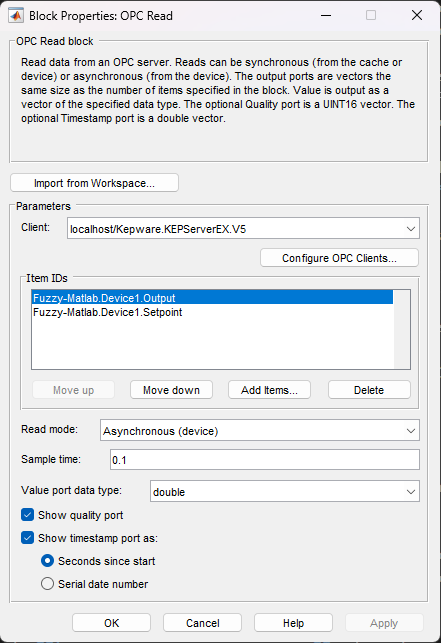
\includegraphics[width=0.5\textwidth]{figuras/imagens/opc-read.png}
    
    {Fonte: Dias, 2025.}
    \label{fig:opcread}
\end{figure}

O \textbf{bloco OPC Write} implementa funcionalidade complementar, permitindo a seleção de tags para escrita de dados da planta para o servidor OPC. As tags configuradas para operação de escrita compreendem \textbf{Error} (erro medido entre setpoint e nível atual), \textbf{Rate} (variação temporal do erro) e \textbf{Level} (nível atual de água no tanque). Esta configuração garante que o cliente OPC UA tenha acesso contínuo às variáveis de processo necessárias para cálculo do controle Fuzzy.

\begin{figure}[H]
    \centering
    \caption[Configuração do bloco OPC Write para escrita de tags no servidor OPC.]{Configuração do bloco OPC Write para escrita de tags no servidor OPC.}
    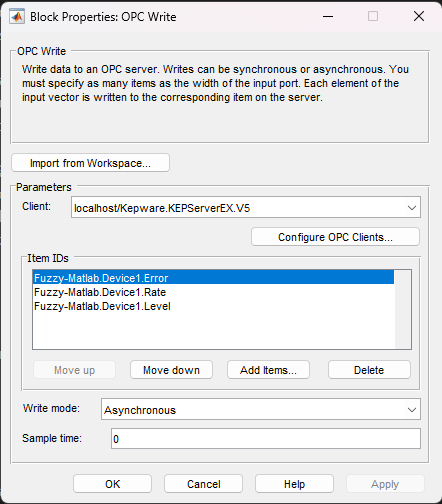
\includegraphics[width=0.5\textwidth]{figuras/imagens/opc-write.png}
    
    {Fonte: Dias, 2025.}
    \label{fig:opcwrite}
\end{figure}

A configuração bidirecional dos blocos OPC Read e OPC Write estabelece ciclo fechado de comunicação entre a planta simulada e o sistema de controle externo. O fluxo de dados iniciado pela escrita das variáveis de processo (Error, Rate, Level) pelo bloco OPC Write é consumido pela API de controle Fuzzy através da IHM, que processa estas informações e retorna comando de controle (Output) juntamente com valor de setpoint atualizado, dados estes lidos pelo bloco OPC Read para atuação na planta.

A estrutura hierárquica do espaço de endereçamento OPC UA implementada segue convenções industriais padrão, organizando as variáveis de processo em namespace específico com identificadores únicos descritivos. A Tabela 1 apresenta o mapeamento completo entre as variáveis de processo e suas respectivas tags OPC UA no servidor.

\begin{table}[H]
\centering
\caption{Mapeamento de variáveis de processo para tags OPC UA}
\begin{adjustbox}{max width=\textwidth}
\begin{tabular}{|l|l|l|l|}
\hline
\textbf{Variável de Processo} & \textbf{Tipo} & \textbf{Tag OPC UA} & \textbf{Descrição} \\
\hline
Error     & Write & Fuzzy-Matlab.Device1.Error     & Erro medido entre setpoint e nível atual \\
Rate      & Write & Fuzzy-Matlab.Device1.Rate      & Variação temporal do erro \\
Level     & Write & Fuzzy-Matlab.Device1.Level     & Nível atual de água no tanque \\
Output    & Read  & Fuzzy-Matlab.Device1.Output    & Saída do valor calculado pela API Fuzzy \\
Setpoint  & Read  & Fuzzy-Matlab.Device1.Setpoint  & Nível de referência para controle \\
\hline
\end{tabular}
\end{adjustbox}
\label{tab:tags-opc-ua}
\end{table}

A nomenclatura adotada utiliza o prefixo \textbf{Fuzzy-Matlab.Device1} seguido pelo identificador específico da variável, proporcionando organização lógica e facilitando identificação das tags pelos clientes OPC UA. Esta estrutura permite expansão futura do sistema através da adição de novos dispositivos (Device2, Device3, etc.) sem conflitos de nomenclatura.

A implementação completa dessas modificações resulta na configuração final da planta mostrada na figura abaixo, onde é possível visualizar a integração dos blocos OPC no modelo original, mantendo a funcionalidade matemática do sistema enquanto adiciona capacidades de comunicação externa padronizada.

\begin{figure}[H]
    \centering
    \caption[Planta de nível modificada com integração OPC UA para comunicação externa.]{Planta de nível modificada com integração OPC UA para comunicação externa.}
    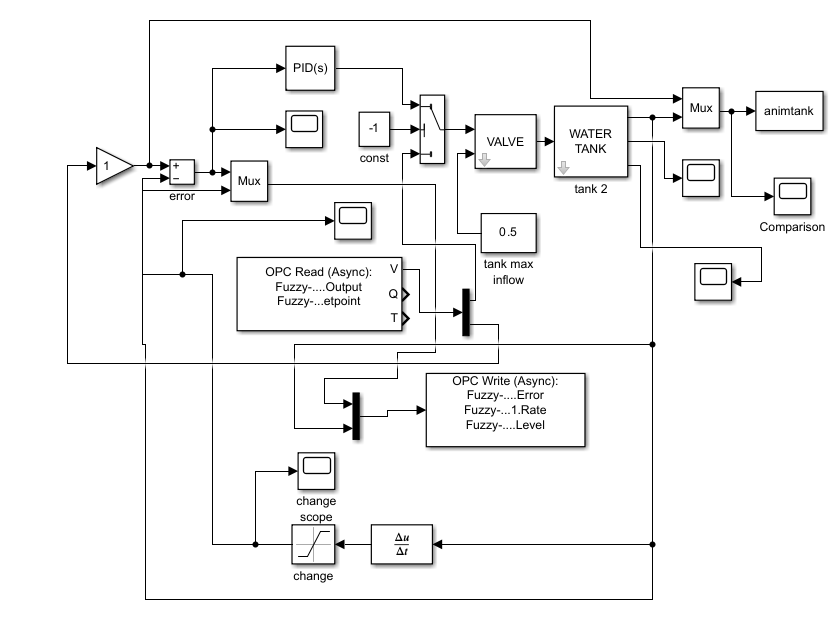
\includegraphics[width=1\textwidth]{figuras/imagens/planta-opc.png}
    
    {Fonte: Dias, 2025.}
    \label{fig:plantaopc}
\end{figure}

\section{Controlador Fuzzy}
\label{sec:controfuzzy}

A lógica Fuzzy representa uma extensão da lógica booleana clássica, permitindo o tratamento de informações imprecisas e incertas através de conjuntos difusos que possibilitam transições graduais entre estados lógicos. Diferentemente da lógica convencional que opera exclusivamente com valores binários (0 ou 1), a lógica Fuzzy admite graus de pertinência intermediários no intervalo [0,1], proporcionando modelagem mais próxima do raciocínio humano e adequada para sistemas complexos com comportamento não linear \cite{zadeh1965}.

O controle Fuzzy fundamenta-se na capacidade de incorporar conhecimento heurístico especializado diretamente no algoritmo de controle, dispensando a necessidade de modelos matemáticos rigorosos do processo. Esta característica torna-se particularmente vantajosa em sistemas de controle de nível, onde não linearidades, tempo morto e variações paramétricas dificultam a aplicação eficaz de técnicas de controle convencionais. A abordagem Fuzzy permite que operadores experientes codifiquem seu conhecimento empírico em regras linguísticas intuitivas, resultando em controladores robustos e de fácil ajuste \cite{mamdani1975}.

A necessidade de implementar o controlador Fuzzy em ambiente Python surge da arquitetura distribuída proposta, onde a lógica de controle opera como serviço independente acessível via API REST. O modelo original \textbf{sltank} do Matlab implementa controle Fuzzy nativo através da ferramenta Fuzzy Logic Designer, sendo necessária a extração e adaptação desses parâmetros para implementação em Python utilizando bibliotecas especializadas como \textbf{scikit-fuzzy}. Esta migração preserva a funcionalidade de controle original enquanto proporciona flexibilidade arquitetural e independência tecnológica \cite{mathWorks2025}.

O controlador Fuzzy implementado utiliza arquitetura de inferência Mamdani com duas variáveis de entrada e uma variável de saída, seguindo a parametrização extraída do exemplo de referência. As \textbf{variáveis de entrada} compreendem o erro de nível (diferença entre setpoint e nível atual) e a taxa de variação do erro (derivada temporal do erro), enquanto a \textbf{variável de saída} corresponde ao sinal de controle da válvula de entrada.

A definição das funções de pertinência segue critérios específicos baseados nas características do processo e na natureza das variáveis envolvidas. As \textbf{variáveis de entrada} (level e rate) utilizam \textbf{funções de pertinência gaussianas}, que proporcionam transições suaves entre os conjuntos difusos e melhor representação da incerteza inerente às medições de processo. As funções gaussianas são caracterizadas pela sua forma em sino, definidas pelos parâmetros de centro e largura, oferecendo gradações naturais que refletem fielmente a imprecisão típica de sensores industriais.

A \textbf{variável de saída} (valve) emprega \textbf{funções de pertinência triangulares}, apropriadas para representar ações de controle discretas e bem definidas. Esta escolha justifica-se pela necessidade de comandos de controle precisos para a válvula, onde a forma triangular proporciona delimitação clara entre diferentes intensidades de atuação, facilitando a interpretação e implementação das ações de controle.

\begin{figure}[H]
    \centering
    \caption[Funções de pertinência gaussianas da variável de entrada "level" (erro de nível).]{Funções de pertinência gaussianas da variável de entrada "level" (erro de nível).}
    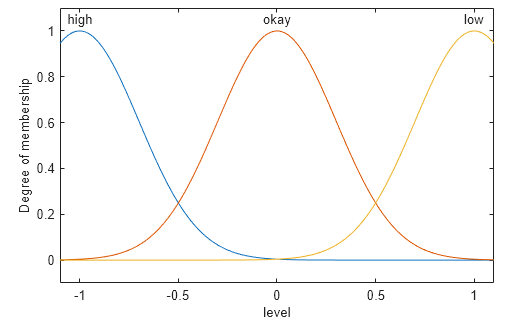
\includegraphics[width=1\textwidth]{figuras/imagens/level.png}
    
    {Fonte: Dias, 2025.}
    \label{fig:fuzzylevel}
\end{figure}

\begin{figure}[H]
    \centering
    \caption[Funções de pertinência gaussianas da variável de entrada "rate" (taxa de variação).]{Funções de pertinência gaussianas da variável de entrada "rate" (taxa de variação).}
    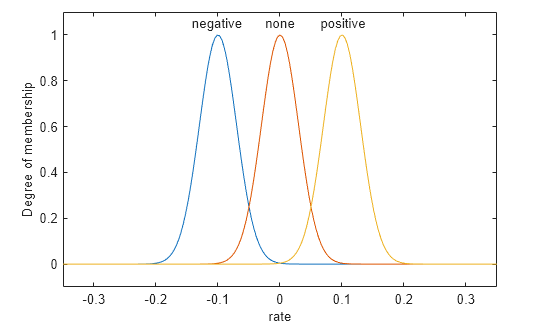
\includegraphics[width=1\textwidth]{figuras/imagens/rate.png}
    
    {Fonte: Dias, 2025.}
    \label{fig:fuzzyrate}
\end{figure}

\begin{figure}[H]
    \centering
    \caption[Funções de pertinência triangulares da variável de saída "valve" (sinal de controle).]{Funções de pertinência triangulares da variável de saída "valve" (sinal de controle).}
    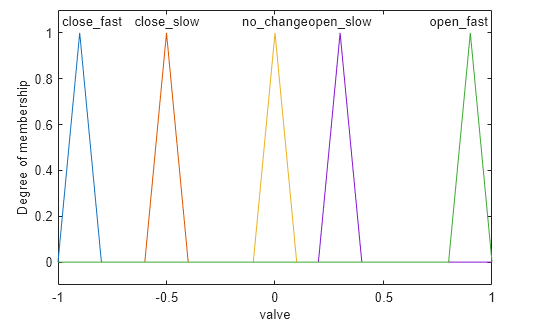
\includegraphics[width=1\textwidth]{figuras/imagens/valve.png}
    
    {Fonte: Dias, 2025.}
    \label{fig:fuzzyvalve}
\end{figure}

O sistema de regras Fuzzy implementado baseia-se em conhecimento heurístico especializado sobre controle de nível, contemplando cinco regras fundamentais que capturam a essência do comportamento desejado do controlador:

\begin{itemize}
\item Regra 1: Se o nível está Ok, então a válvula não é ajustada (\( \sigma \): 0,3; \( \mu \): 0)
Esta regra estabelece a condição de equilíbrio, onde pequenos desvios em torno do setpoint não resultam em ações de controle significativas, evitando oscilações desnecessárias e garantindo estabilidade em regime permanente. Os parâmetros da função gaussiana definem um desvio padrão de 0,3 centrado em zero.
\item Regra 2: Se o nível está Low, então abra a válvula rapidamente (\( \sigma \): 0,3; \( \mu \): 1)
Implementa ação corretiva intensa para situações de nível baixo, aumentando significativamente a vazão de entrada para recuperação rápida do nível desejado, priorizando a segurança operacional e evitando operação em vazio. A função gaussiana apresenta desvio padrão de 0,3 centrada em 1.
\item Regra 3: Se o nível está High, então feche-a rapidamente (\( \sigma \): 0,3; \( \mu \): -1)
Estabelece resposta imediata para condições de nível elevado, reduzindo drasticamente a vazão de entrada para prevenir transbordamentos e manter o processo dentro dos limites operacionais seguros. A parametrização gaussiana utiliza desvio padrão de 0,3 centrado em -1.
\item Regra 4: Se o nível está Ok e aumentando, então feche a válvula devagar
Incorpora comportamento antecipativo baseado na taxa de variação, aplicando correção preventiva quando o nível aproxima-se do setpoint com tendência ascendente, evitando ultrapassagem excessiva.
\item Regra 5: Se o nível está Ok e decrescendo, então abra a válvula devagar
Complementa o comportamento antecipativo para tendência descendente, proporcionando correção suave quando o nível está próximo do setpoint mas apresenta tendência de redução.
\end{itemize}

onde, 

\begin{itemize}
    \item \( \sigma \) é o desvio padrão (sigma) das funções de pertinência gaussianas.
    \item \( \mu \) é o valor médio (mu) das funções de pertinência gaussianas.
\end{itemize}

Esta estrutura de regras implementa estratégia de controle híbrida que combina \textbf{ação corretiva proporcional} ao erro medido com \textbf{comportamento antecipativo} baseado na derivada temporal, resultando em controlador robusto capaz de lidar eficazmente com as características não lineares do processo de controle de nível.

\section{API de controle Fuzzy}
\label{sec:apicontrolefuzzy}

A implementação da API de controle Fuzzy constitui o núcleo computacional inteligente da arquitetura distribuída proposta, responsável por materializar os conceitos teóricos de lógica Fuzzy em uma aplicação prática acessível via protocolo HTTP/REST. Esta API representa a tradução dos parâmetros e regras definidos anteriormente em código Python executável, proporcionando interface padronizada para integração com sistemas industriais heterogêneos.

A escolha do padrão arquitetural REST (Representational State Transfer) para a API justifica-se pela necessidade de criar uma interface de comunicação independente de plataforma, permitindo que diferentes clientes possam consumir os serviços de controle sem dependência de tecnologias específicas. Esta abordagem facilita a integração da lógica de controle Fuzzy com sistemas existentes, desde aplicações desktop desenvolvidas em C\# até sistemas embarcados ou aplicações web modernas.

A implementação do controlador Fuzzy em Python utiliza a biblioteca \textbf{scikit-fuzzy} para materializar os conceitos teóricos apresentados anteriormente. O código desenvolvido define as variáveis de entrada e saída com seus respectivos universos de discurso, implementa as funções de pertinência gaussianas e triangulares, e estabelece as regras de inferência que governam o comportamento do controlador:

\begin{center}
\begin{lstlisting}[language=Python, caption=Código Python para controle Fuzzy]
import numpy as np
import skfuzzy as fuzz
from skfuzzy import control as ctrl

level = ctrl.Antecedent(np.arange(-1.1, 1.1, 0.001), 'level')
rate = ctrl.Antecedent(np.arange(-0.35, 0.35, 0.001), 'rate')
valve = ctrl.Consequent(np.arange(-1, 1, 0.001), 'valve')

level['high'] = fuzz.gaussmf(level.universe, -1, 0.3)
level['okay'] = fuzz.gaussmf(level.universe, 0, 0.3)
level['low'] = fuzz.gaussmf(level.universe, 1, 0.3)

rate['negative'] = fuzz.gaussmf(rate.universe, -0.1, 0.03)
rate['none'] = fuzz.gaussmf(rate.universe, 0, 0.03)
rate['positive'] = fuzz.gaussmf(rate.universe, 0.1, 0.03)

valve['close_fast'] = fuzz.trimf(valve.universe, [-1, -0.9, -0.8])
valve['close_slow'] = fuzz.trimf(valve.universe, [-0.6, -0.5, -0.4])
valve['no_change'] = fuzz.trimf(valve.universe, [-0.1, 0, 0.1])
valve['open_slow'] = fuzz.trimf(valve.universe, [0.2, 0.3, 0.4])
valve['open_fast'] = fuzz.trimf(valve.universe, [0.8, 0.9, 1])

rule1 = ctrl.Rule(level['okay'], valve['no_change'])
rule2 = ctrl.Rule(level['low'], valve['open_fast'])
rule3 = ctrl.Rule(level['high'], valve['close_fast'])
rule4 = ctrl.Rule(level['okay'] & rate['positive'], valve['close_slow'])
rule5 = ctrl.Rule(level['okay'] & rate['negative'], valve['open_slow'])
\end{lstlisting}
\end{center}

A estrutura do código reflete diretamente os conceitos teóricos estabelecidos no capítulo \ref{sec:controfuzzy}, onde as variáveis de entrada `evel e rate utilizam funções de pertinência gaussianas com parâmetros específicos extraídos do modelo de referência do MathWorks. A variável de saída valve emprega funções triangulares que proporcionam ações de controle bem definidas, facilitando a interpretação e implementação dos comandos de atuação na válvula.

As cinco regras de inferência implementadas capturam o conhecimento heurístico especializado sobre controle de nível, estabelecendo relações lógicas entre as variáveis de entrada e a ação de controle resultante. Esta implementação preserva a funcionalidade do controlador original enquanto proporciona flexibilidade para integração em arquiteturas distribuídas através da API REST.

A API desenvolvida estrutura-se em três endpoints principais sob a rota base \textbf{api/}, proporcionando funcionalidades específicas para diferentes aspectos do sistema de controle:

\textbf{Endpoint /health (GET)}: Implementa verificação de saúde da API, permitindo que sistemas externos monitorem o status operacional do serviço de controle Fuzzy. Este endpoint retorna informações sobre a disponibilidade e funcionamento correto da API, facilitando implementação de estratégias de monitoramento e recuperação automática em caso de falhas.

Exemplo de requisição:

\begin{verbatim}
GET /api/health
\end{verbatim}

Exemplo de resposta:

\begin{center}
\begin{verbatim}
{
  "status": "healthy",
  "message": "API is running correctly"
}
\end{verbatim}
\end{center}

\textbf{Endpoint /valve-opening (POST)}: Constitui o núcleo funcional da API, responsável pela aplicação da lógica Fuzzy às variáveis de processo recebidas. Aceita requisições JSON contendo as propriedades level (erro de nível) e rate (taxa de variação do erro), processa estas informações através do sistema de inferência Mamdani implementado e retorna resposta JSON com a propriedade valve\_opening, representando o sinal de controle calculado para atuação na válvula.

Exemplo de requisição:

\begin{verbatim}
POST /api/valve-opening
Content-Type: application/json

{
  "level": 0.3,
  "rate": -0.05
}
\end{verbatim}

Exemplo de resposta:

\begin{center}
\begin{verbatim}
{
  "valve_opening": 0.42
}
\end{verbatim}
\end{center}

\textbf{Endpoint /performance-metrics (POST)}: Proporciona funcionalidade de análise de desempenho do sistema de controle, calculando métricas quantitativas para avaliação da eficácia do controlador Fuzzy. Recebe requisições JSON contendo ref (valor de referência, tipicamente entre 0.5 e 1.5), tol (tolerância para cálculo do tempo de acomodação), y (array de valores de nível medidos) e t (array de valores temporais correspondentes). Os arrays y e t devem possuir o mesmo tamanho para garantir correspondência entre valores temporais e medições de nível. O endpoint retorna objeto JSON contendo as propriedades mse (erro quadrático médio), overshoot (sobressinal percentual) e settling\_time (tempo de acomodação), facilitando a validação e otimização do desempenho do sistema integrado.

Exemplo de requisição:

\begin{verbatim}
POST /api/performance-metrics
Content-Type: application/json

{
  "ref": 1.0,
  "tol": 0.02,
  "y": [0.0, 0.2, 0.5, 0.8, 0.95, 1.05, 1.02, 1.0, 0.98, 1.0],
  "t": [0.0, 1.0, 2.0, 3.0, 4.0, 5.0, 6.0, 7.0, 8.0, 9.0]

\end{verbatim}

Exemplo de resposta:

\begin{center}
\begin{verbatim}
{
  "mse": 0.0245,
  "overshoot": 5.2,
  "settling_time": 6.5
}
\end{verbatim}
\end{center}

\section{IHM e cliente OPC UA}
\label{sec:ihmeopc}

A Interface Humano-Máquina (IHM) integrada ao cliente OPC UA constitui o elemento centralizador da arquitetura distribuída proposta, atuando como ponte de comunicação entre todos os componentes do sistema de controle. Esta aplicação desktop desenvolvida em C\# desempenha papel fundamental na coordenação do fluxo de dados entre a planta de nível simulada, a API de controle Fuzzy e o operador humano, proporcionando supervisão em tempo real e capacidade de intervenção manual no processo.

A escolha da linguagem C\# para desenvolvimento da IHM justifica-se por sua robustez na criação de aplicações desktop nativas do Windows, ampla disponibilidade de bibliotecas especializadas para comunicação OPC UA e facilidade de integração com APIs REST através de requisições HTTP. O framework .NET proporciona recursos avançados para desenvolvimento de interfaces gráficas responsivas e funcionais, essenciais para operação eficiente em ambiente industrial.

A arquitetura dual da aplicação implementa simultaneamente funcionalidades de cliente OPC UA para comunicação com a planta simulada e cliente HTTP para consumo dos serviços da API de controle Fuzzy. Esta abordagem permite que a IHM atue como elemento coordenador do sistema, recebendo dados de processo via OPC UA, processando-os através da API Fuzzy e retornando os comandos de controle para atuação na planta, fechando o ciclo de controle distribuído.

\begin{figure}[H]
    \centering
    \caption[Interface Humano-Máquina integrada com cliente OPC UA para supervisão e controle.]{Interface Humano-Máquina integrada com cliente OPC UA para supervisão e controle.}
    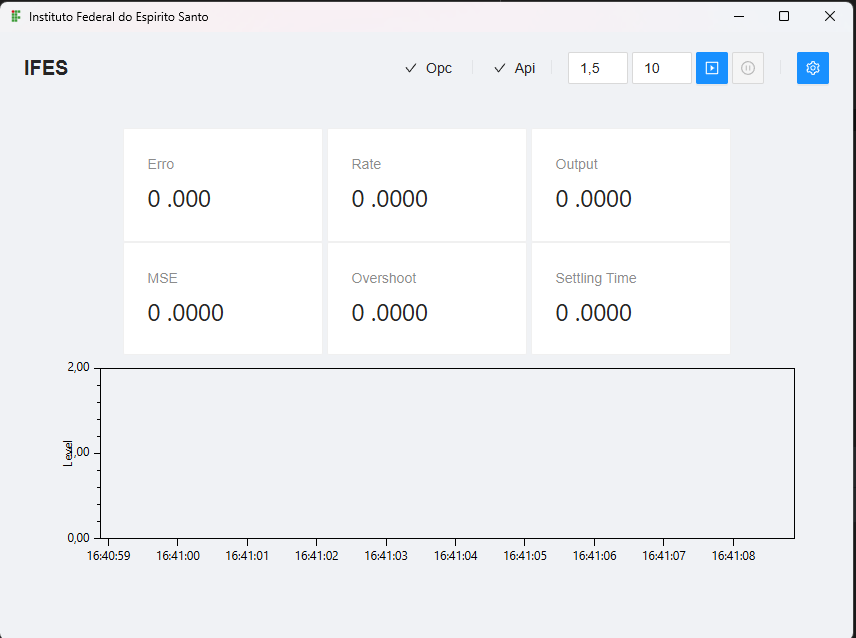
\includegraphics[width=1\textwidth]{figuras/imagens/ihm.png}
    
    {Fonte: Dias, 2025.}
    \label{fig:ihm}
\end{figure}

A IHM desenvolvida incorpora funcionalidades abrangentes de configuração e operação, proporcionando flexibilidade e facilidade de uso para diferentes cenários de aplicação. O sistema de configuração OPC permite ao usuário definir dinamicamente a URL do servidor OPC UA e especificar as tags de comunicação correspondentes às variáveis de processo. Esta funcionalidade elimina a necessidade de recompilação da aplicação para diferentes configurações de planta, facilitando a adaptação a diversos ambientes industriais e proporcionando portabilidade do sistema.

\begin{figure}[H]
    \centering
    \caption[Configuração do cliente OPC UA na interface da IHM.]{Configuração do cliente OPC UA na interface da IHM.}
    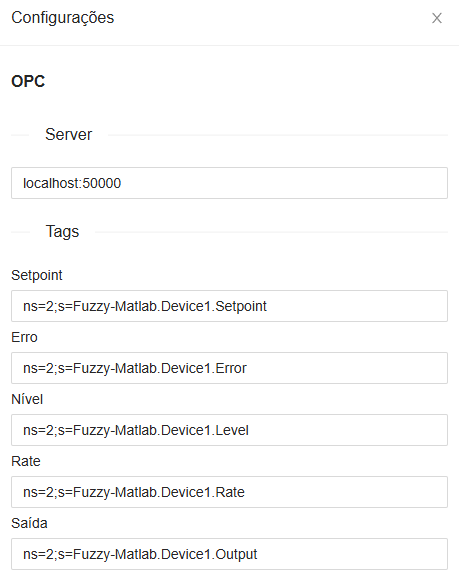
\includegraphics[width=0.7\textwidth]{figuras/imagens/ihm-config-opc.png}
    
    {Fonte: Dias, 2025.}
    \label{fig:ihmconfigopc}
\end{figure}

A interface oferece configuração do endpoint da API de controle Fuzzy, permitindo que o operador especifique o endereço do servidor onde a API está hospedada. Esta flexibilidade arquitetural possibilita distribuição geográfica dos componentes do sistema, onde a API pode operar em servidores dedicados ou em nuvem, enquanto a IHM mantém comunicação através de requisições HTTP padronizadas. A configuração dinâmica do endpoint facilita implementação em diferentes topologias de rede e estratégias de implantação.

\begin{figure}[H]
    \centering
    \caption[Configuração do endpoint da API de controle Fuzzy.]{Configuração do endpoint da API de controle Fuzzy.}
    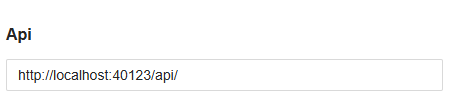
\includegraphics[width=0.7\textwidth]{figuras/imagens/ihm-config-api.png}
    
    {Fonte: Dias, 2025.}
    \label{fig:ihmconfigapi}
\end{figure}

O módulo de simulação integrado constitui funcionalidade essencial para validação e teste do sistema de controle. A IHM permite ao usuário definir o nível desejado (setpoint) e especificar o tempo de simulação em segundos, iniciando automaticamente o processo de controle com os parâmetros estabelecidos. Esta capacidade de simulação facilita análise de comportamento do sistema, otimização de parâmetros de controle e treinamento de operadores sem necessidade de intervenção direta na planta física.

\begin{figure}[H]
    \centering
    \caption[Interface de simulação integrada para testes do sistema de controle.]{Interface de simulação integrada para testes do sistema de controle.}
    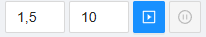
\includegraphics[]{figuras/imagens/ihm-simulation.png}
    
    {Fonte: Dias, 2025.}
    \label{fig:ihmsimulation}
\end{figure}

A visualização do status de conexão proporciona monitoramento contínuo da integridade das comunicações com o servidor OPC UA e a API de controle Fuzzy. Indicadores visuais em tempo real informam sobre o estado das conexões, facilitando identificação rápida de problemas de comunicação e implementação de estratégias de recuperação automática. Esta funcionalidade é fundamental para operação confiável em ambiente industrial, onde a continuidade da comunicação impacta diretamente a segurança e eficiência do processo.

\begin{figure}[H]
    \centering
    \caption[Monitoramento do status de conexão com servidor OPC UA e API.]{Monitoramento do status de conexão com servidor OPC UA e API.}
    
\includegraphics[]{figuras/imagens/ihm-service-status.png}
    
    {Fonte: Dias, 2025.}
    \label{fig:ihmsimulation}
\end{figure}

A interface gráfica integra todos estes elementos em layout intuitivo e funcional, proporcionando ao operador controle completo sobre o sistema distribuído através de uma única aplicação centralizada. A combinação destas funcionalidades resulta em ferramenta robusta para supervisão, controle e análise do sistema de controle de nível baseado em lógica Fuzzy integrado via protocolo OPC UA.
  \chapter{Resultados e Discussão}
\label{cap:resultadosediscussao}

Este capítulo apresenta os resultados obtidos através da implementação e integração da arquitetura distribuída de controle de nível baseada em lógica Fuzzy utilizando protocolo OPC UA. A análise compreende a avaliação sistemática do desempenho do sistema integrado, comparando os resultados do controlador Fuzzy distribuído com implementações de referência e estabelecendo métricas quantitativas para validação da eficácia da arquitetura proposta.

A metodologia de avaliação fundamenta-se na execução de testes controlados utilizando a planta de nível simulada do Matlab/Simulink, onde o controlador Fuzzy implementado em Python através da API REST é comparado com o controlador Fuzzy nativo do ambiente Matlab. Esta abordagem comparativa permite quantificar o impacto da distribuição dos componentes do sistema no desempenho de controle, identificando potenciais perdas de eficiência decorrentes da comunicação via protocolo OPC UA e requisições HTTP.

\section{Avaliação de Desempenho do Controlador Fuzzy Nativo}
\label{sec:fuzzynativo}

O primeiro conjunto de experimentos concentra-se na validação do sistema de controle utilizando o controlador Fuzzy nativo integrado à planta simulada do Matlab/Simulink, estabelecendo uma linha de base para comparação com a arquitetura distribuída proposta. Esta etapa fundamental visa caracterizar o desempenho de referência do sistema de controle, quantificando métricas como tempo de acomodação, sobressinal e erro em regime permanente sob condições operacionais controladas.

A configuração experimental utiliza o controlador Fuzzy original implementado através da ferramenta Fuzzy Logic Designer do Matlab, preservando todos os parâmetros de função de pertinência, universos de discurso e regras de inferência estabelecidos no modelo de referência. Esta abordagem garante que os resultados obtidos reflitam exclusivamente o desempenho do algoritmo de controle Fuzzy, sem influência de fatores relacionados à comunicação em rede ou processamento distribuído.

Para possibilitar a visualização e monitoramento através da IHM desenvolvida, foi necessário implementar modificações estruturais na planta original, adicionando blocos de comunicação OPC UA para exposição das variáveis de processo. Estas modificações mantêm a integridade do modelo matemático da planta enquanto proporcionam interface padronizada para supervisão external, conforme apresentado na figura seguinte.

\begin{figure}[H]
    \centering
    \caption[Configuração da planta de nível com controlador Fuzzy nativo e comunicação OPC.]{Configuração da planta de nível com controlador Fuzzy nativo e comunicação OPC.}
    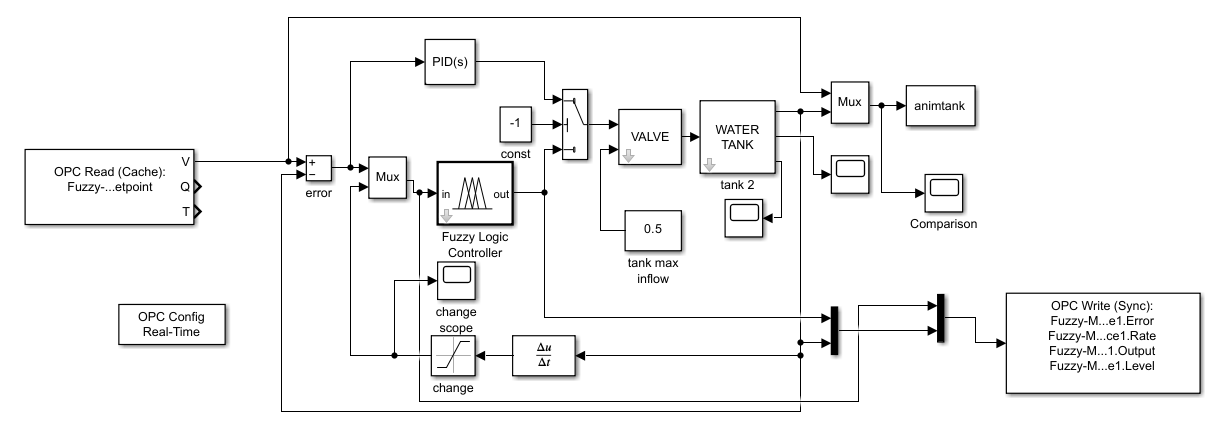
\includegraphics[width=1\textwidth]{figuras/testes/sem-integracao/planta.png}
    
    {Fonte: Dias, 2025.}
    \label{fig:testeplanta}
\end{figure}

A metodologia experimental compreende três cenários de teste distintos, cada um projetado para avaliar o comportamento do controlador Fuzzy em diferentes faixas operacionais da planta de nível. Os testes são conduzidos com duração de 50 segundos, proporcionando tempo adequado para análise completa da resposta transitória e atingimento do regime permanente. A coleta de dados inclui métricas quantitativas essenciais: erro quadrático médio (MSE), sobressinal percentual e tempo de acomodação, este último calculado com tolerância de 2\% (0,02) para operações de enchimento do tanque e 3\% (0,03) para operações de esvaziamento.

A diferenciação das tolerâncias fundamenta-se nas características assimétricas inerentes ao modelo de tanque utilizado, conforme documentado pela MathWorks (2025). Devido ao diâmetro do tubo de saída, o tanque esvazia mais lentamente do que se enche, criando dinâmicas distintas que requerem tratamento diferenciado. Esta assimetria é compensada no sistema Fuzzy através de funções de pertinência não simétricas para as ações \textbf{close\_slow} e \textbf{open\_slow}, uma característica que controladores PID convencionais não suportam adequadamente.

\textbf{Teste 1}: Transição de 0 para 0,5 metros.

O primeiro experimento avalia o comportamento do sistema partindo de condição inicial de tanque vazio até nível intermediário de 0,5 metros, representando cenário crítico de partida do processo. Os resultados obtidos demonstram desempenho satisfatório com MSE de 0,02, indicando baixo erro acumulado durante a resposta transitória. O sobressinal negativo de -0,0092 evidencia comportamento conservador do controlador, evitando ultrapassagem do setpoint. O tempo de acomodação de 31,2166 segundos reflete a dinâmica natural do sistema para grandes variações de nível.

\begin{figure}[H]
    \centering
    \caption[Resposta do sistema para transição de nível 0→0,5m com controlador Fuzzy nativo.]{Resposta do sistema para transição de nível 0→0,5m com controlador Fuzzy nativo.}
    
\includegraphics[width=1\textwidth]{figuras/testes/sem-integracao/zero-to-zero-dot-five.png}
    
    {Fonte: Dias, 2025.}
\end{figure}

\textbf{Teste 2}: Transição de 0,5 para 1,0 metro.

O segundo experimento analisa o comportamento em faixa operacional intermediária, avaliando a resposta do controlador para variação de setpoint de 0,5 para 1,0 metro. Os resultados indicam MSE de 0,0231, ligeiramente superior ao teste anterior devido à maior complexidade dinâmica nesta faixa operacional. O sobressinal negativo de -0,0057 mantém o padrão conservador, enquanto o tempo de acomodação reduzido para 20,2013 segundos demonstra melhor resposta dinâmica em níveis intermediários.

\begin{figure}[H]
    \centering
    \caption[Resposta do sistema para transição de nível 0,5→1,0m com controlador Fuzzy nativo.]{Resposta do sistema para transição de nível 0,5→1,0m com controlador Fuzzy nativo.}
    
\includegraphics[width=1\textwidth]{figuras/testes/sem-integracao/zero-dot-five-to-one.png}
    
    {Fonte: Dias, 2025.}
\end{figure}

\textbf{Teste 3}: Transição de 1,0 para 1,5 metros.

O terceiro experimento examina o comportamento em faixa operacional superior, com transição de 1,0 para 1,5 metros, avaliando a eficácia do controlador em níveis elevados do tanque. Os resultados mostram MSE de 0,0224, comparável ao teste anterior, indicando consistência de desempenho. O sobressinal negativo mínimo de -0,0034 sugere maior precisão na aproximação ao setpoint, enquanto o tempo de acomodação otimizado de 17,3841 segundos evidencia resposta mais rápida em níveis superiores.

\begin{figure}[H]
    \centering
    \caption[Resposta do sistema para transição de nível 1,0→1,5m com controlador Fuzzy nativo.]{Resposta do sistema para transição de nível 1,0→1,5m com controlador Fuzzy nativo.}
    
\includegraphics[width=1\textwidth]{figuras/testes/sem-integracao/one-to-one-dot-five.png}
    
    {Fonte: Dias, 2025.}
\end{figure}

A análise comparativa dos três experimentos revela características importantes do comportamento do controlador Fuzzy nativo. O tempo de acomodação apresenta tendência decrescente com o aumento do nível operacional (31,22s → 20,20s → 17,38s), sugerindo melhor resposta dinâmica em níveis mais elevados. O MSE mantém-se consistentemente baixo (0,02 a 0,0231), demonstrando precisão adequada em todas as faixas operacionais. Os valores negativos de sobressinal confirmam estratégia conservadora do controlador, priorizando estabilidade sobre rapidez de resposta.

\textbf{Teste 4}: Transição de 1,5 para 1,0 metro.

O quarto experimento avalia o comportamento do sistema durante operação de esvaziamento, com transição de 1,5 para 1,0 metro, representando o primeiro teste de redução de nível na análise experimental. Os resultados demonstram características distintas das operações de enchimento, com MSE de 0,0163, valor inferior aos testes anteriores, indicando maior precisão durante o esvaziamento. O sobressinal positivo de 0,0206 contrasta com o padrão conservador dos testes de enchimento, evidenciando a assimetria inerente ao sistema. O tempo de acomodação de 12,8298 segundos confirma a dinâmica mais rápida para operações de esvaziamento em níveis superiores.

\begin{figure}[H]
    \centering
    \caption[Resposta do sistema para transição de nível 1,5→1,0m com controlador Fuzzy nativo.]{Resposta do sistema para transição de nível 1,5→1,0m com controlador Fuzzy nativo.}
    
\includegraphics[width=1\textwidth]{figuras/testes/sem-integracao/one-dot-five-to-one.png}
    
    {Fonte: Dias, 2025.}
\end{figure}

\textbf{Teste 5}: Transição de 1,0 para 0,5 metros.

O quinto experimento analisa o comportamento durante esvaziamento em faixa operacional intermediária, com transição de 1,0 para 0,5 metros, complementando a análise de redução de nível iniciada no teste anterior. Os resultados mostram MSE de 0,0162, mantendo a tendência de maior precisão durante operações de esvaziamento. O sobressinal positivo de 0,0138, menor que o teste anterior, sugere melhor controle da aproximação ao setpoint em níveis intermediários. O tempo de acomodação de 14,8411 segundos, ligeiramente superior ao teste 4, reflete a dinâmica específica desta faixa operacional durante esvaziamento.

\begin{figure}[H]
    \centering
    \caption[Resposta do sistema para transição de nível 1,0→0,5m com controlador Fuzzy nativo.]{Resposta do sistema para transição de nível 1,0→0,5m com controlador Fuzzy nativo.}
    
\includegraphics[width=1\textwidth]{figuras/testes/sem-integracao/one-to-zero-dot-five.png}
    
    {Fonte: Dias, 2025.}
\end{figure}

A análise integrada dos cinco experimentos evidencia comportamentos assimétricos fundamentais do sistema de controle de nível. Os testes de enchimento (1-3) apresentam sobressinais negativos e tempos de acomodação decrescentes com o aumento do nível (31,22s → 20,20s → 17,38s), enquanto os testes de esvaziamento (4-5) demonstram sobressinais positivos e tempos de acomodação reduzidos (12,83s e 14,84s). O MSE apresenta valores consistentemente baixos em ambas as operações, com ligeira superioridade durante esvaziamento (0,0162-0,0163) comparado ao enchimento (0,02-0,0231), confirmando a eficácia das funções de pertinência assimétricas implementadas no controlador Fuzzy.

\section{Avaliação de Desempenho da Arquitetura Distribuída via API REST}
\label{sec:fuzzydistribuido}

O segundo conjunto de experimentos avalia o desempenho do sistema de controle utilizando a arquitetura distribuída proposta, onde o controlador Fuzzy é implementado como serviço web independente em Python, comunicando-se com a planta simulada através do protocolo OPC UA e requisições HTTP REST. Esta configuração representa o núcleo da contribuição técnica do presente trabalho, integrando tecnologias modernas de comunicação industrial com algoritmos de controle inteligente.

A arquitetura distribuída introduz complexidade adicional ao sistema de controle através da separação física e lógica dos componentes, criando uma cadeia de comunicação que compreende: (1) leitura de variáveis de processo via OPC UA, (2) transmissão de dados através de requisições HTTP POST para a API Python, (3) processamento do algoritmo Fuzzy no servidor web, (4) retorno do sinal de controle via resposta HTTP, e (5) escrita do sinal de controle na planta via OPC UA. Esta separação permite maior flexibilidade de implementação, facilita a manutenção e atualizações do controlador, e possibilita a integração com sistemas de supervisão corporativos.

O objetivo fundamental desta etapa experimental é quantificar o impacto da latência de comunicação e do processamento distribuído no desempenho de controle, comparando diretamente as métricas obtidas com os resultados do controlador nativo estabelecidos na seção anterior. A metodologia experimental mantém os mesmos cenários de teste (transições 0→0,5m, 0,5→1,0m e 1,0→1,5m) e parâmetros de simulação, garantindo comparabilidade direta entre as duas abordagens.

A configuração experimental utiliza a Interface Humano-Máquina desenvolvida em C\# como elemento central de orquestração, integrando simultaneamente o cliente OPC UA para comunicação com a planta simulada e o cliente HTTP para requisições à API REST do controlador Fuzzy. Esta implementação demonstra a viabilidade prática da arquitetura distribuída em ambiente industrial, onde diferentes subsistemas devem operar de forma coordenada e confiável.

\textbf{Teste 1}: Transição de 0 para 0,5 metros - Arquitetura Distribuída.

O primeiro experimento utilizando a arquitetura distribuída avalia o comportamento do sistema para transição de tanque vazio até nível intermediário de 0,5 metros, replicando as condições do teste de referência. Os resultados demonstram MSE de 0,0174, ligeiramente superior ao controlador nativo (0,02), indicando impacto mínimo da latência de comunicação. O sobressinal negativo de -0,0102 mantém o padrão conservador, enquanto o tempo de acomodação de 31,9768 segundos apresenta aumento de apenas 2,4\% comparado ao sistema nativo, evidenciando eficácia da arquitetura distribuída.

\begin{figure}[H]
    \centering
    \caption[Resposta do sistema para transição de nível 0→0,5m com arquitetura distribuída via API REST.]{Resposta do sistema para transição de nível 0→0,5m com arquitetura distribuída via API REST.}
    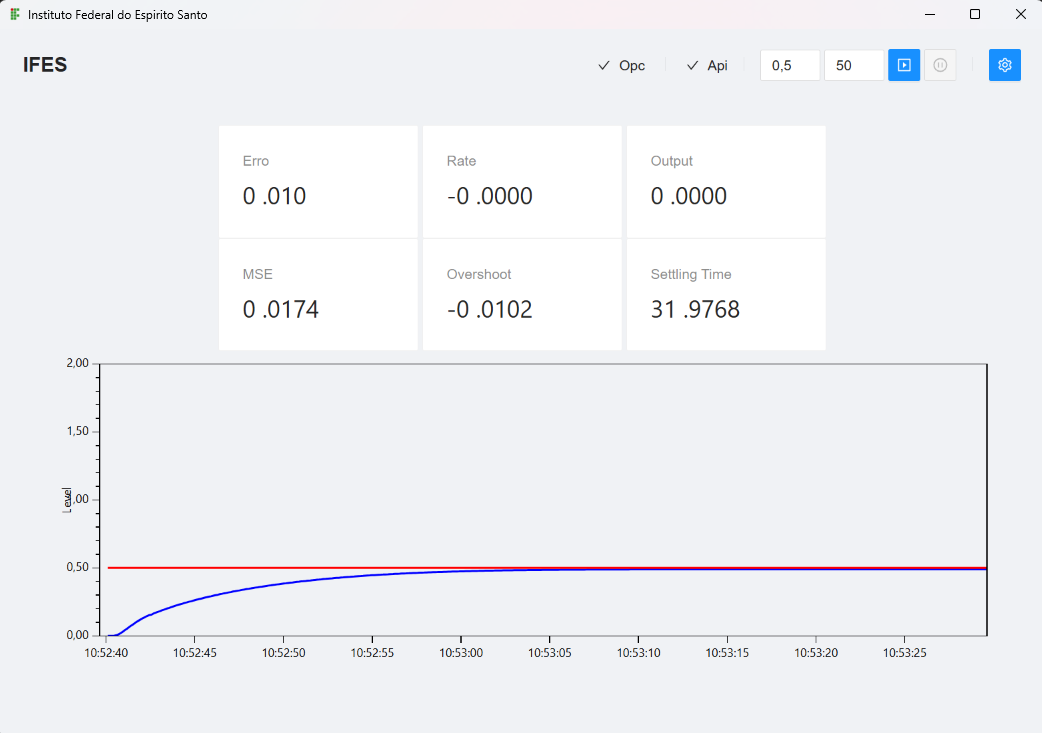
\includegraphics[width=1\textwidth]{figuras/testes/com-integracao/zero-to-zero-dot-five.png}
    
    {Fonte: Dias, 2025.}
\end{figure}

\textbf{Teste 2}: Transição de 0,5 para 1,0 metro - Arquitetura Distribuída.

O segundo experimento com arquitetura distribuída analisa a resposta para transição de 0,5 para 1,0 metro, permitindo comparação direta com o controlador nativo. Os resultados mostram MSE de 0,0140, valor inferior ao sistema nativo (0,0231), indicando desempenho superior da arquitetura distribuída nesta faixa operacional. O sobressinal negativo de -0,0097 mantém características conservadoras, enquanto o tempo de acomodação de 18,9734 segundos demonstra melhoria de 6,1\% comparado ao sistema de referência.

\begin{figure}[H]
    \centering
    \caption[Resposta do sistema para transição de nível 0,5→1,0m com arquitetura distribuída via API REST.]{Resposta do sistema para transição de nível 0,5→1,0m com arquitetura distribuída via API REST.}
    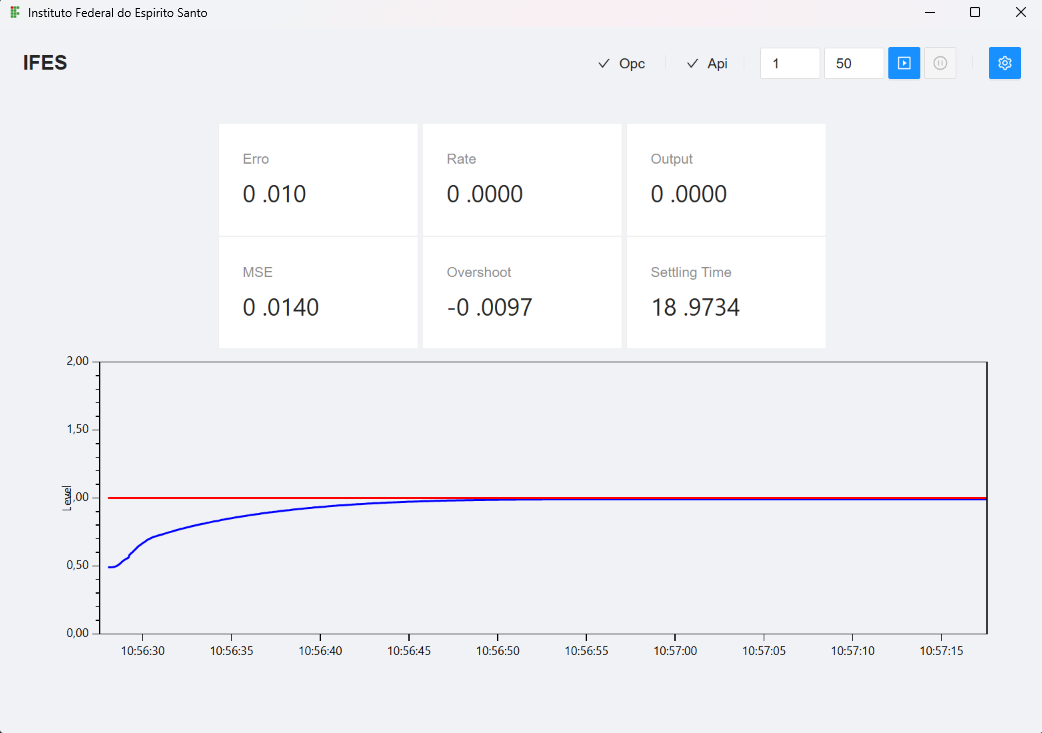
\includegraphics[width=1\textwidth]{figuras/testes/com-integracao/zero-dot-five-to-one.png}
    
    {Fonte: Dias, 2025.}
\end{figure}

\textbf{Teste 3}: Transição de 1,0 para 1,5 metros - Arquitetura Distribuída.

O terceiro experimento avalia o comportamento em faixa operacional superior utilizando a arquitetura distribuída, com transição de 1,0 para 1,5 metros. Os resultados apresentam MSE de 0,0150, valor comparável ao controlador nativo (0,0224), demonstrando consistência de desempenho. O sobressinal negativo de -0,0093 confirma estratégia conservadora, enquanto o tempo de acomodação de 16,2892 segundos representa melhoria de 6,2\% em relação ao sistema nativo, evidenciando vantagens da implementação distribuída em níveis elevados.

\begin{figure}[H]
    \centering
    \caption[Resposta do sistema para transição de nível 1,0→1,5m com arquitetura distribuída via API REST.]{Resposta do sistema para transição de nível 1,0→1,5m com arquitetura distribuída via API REST.}
    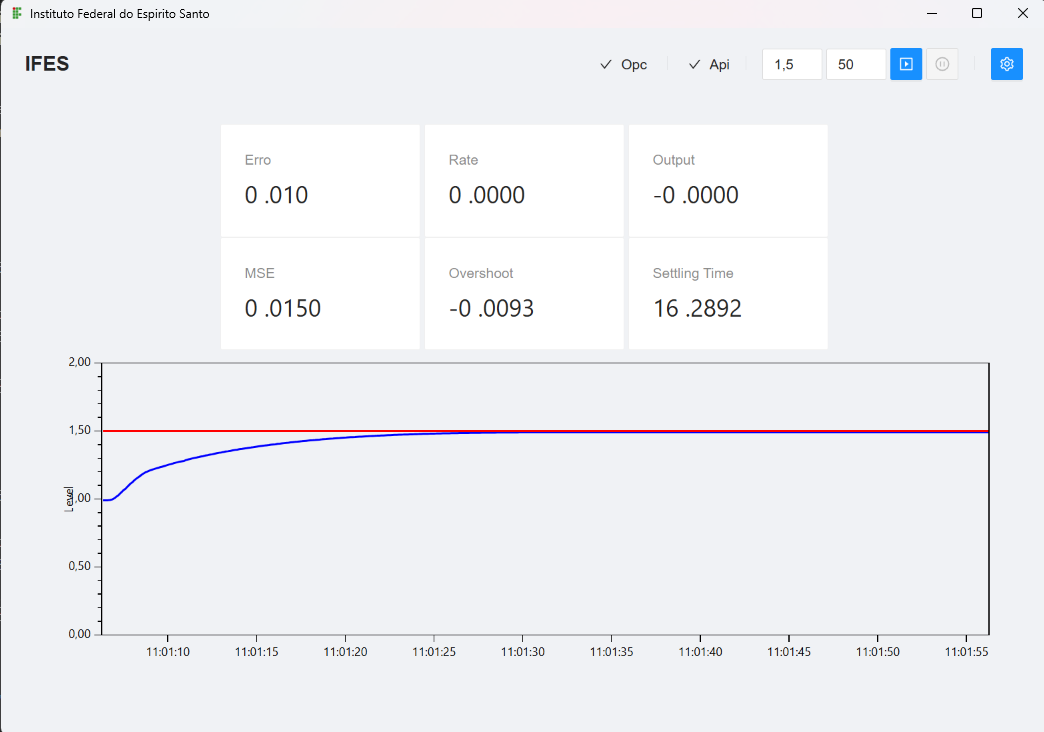
\includegraphics[width=1\textwidth]{figuras/testes/com-integracao/one-to-one-dot-five.png}
    
    {Fonte: Dias, 2025.}
\end{figure}

A análise dos três primeiros experimentos de enchimento com arquitetura distribuída revela desempenho notavelmente superior ao sistema nativo. O MSE apresenta valores consistentemente menores (0,0174 → 0,0140 → 0,0150) comparados ao controlador nativo (0,02 → 0,0231 → 0,0224), demonstrando maior precisão da implementação distribuída. Os tempos de acomodação mostram melhoria progressiva: ligeiro aumento de 2,4\% no teste 1, seguido por melhorias significativas de 6,1\% e 6,2\% nos testes 2 e 3, respectivamente. Os sobressinais negativos mantêm-se consistentes (-0,0102 → -0,0097 → -0,0093), preservando a estratégia conservadora do controlador original enquanto demonstram maior estabilidade que o sistema nativo.

\textbf{Teste 4}: Transição de 1,5 para 1,0 metro - Arquitetura Distribuída.

O quarto experimento utilizando arquitetura distribuída avalia operações de esvaziamento, com transição de 1,5 para 1,0 metro, estabelecendo comparação com o primeiro teste de esvaziamento do sistema nativo. Os resultados demonstram MSE de 0,0105, valor significativamente inferior ao controlador nativo (0,0163), indicando maior precisão da arquitetura distribuída durante esvaziamento. Notavelmente, o sobressinal apresenta valor negativo (-0,0121), contrastando com o padrão positivo do sistema nativo, sugerindo comportamento mais conservador. O tempo de acomodação de 10,8028 segundos representa melhoria de 15,8\% comparado ao sistema de referência.

\begin{figure}[H]
    \centering
    \caption[Resposta do sistema para transição de nível 1,5→1,0m com arquitetura distribuída via API REST.]{Resposta do sistema para transição de nível 1,5→1,0m com arquitetura distribuída via API REST.}
    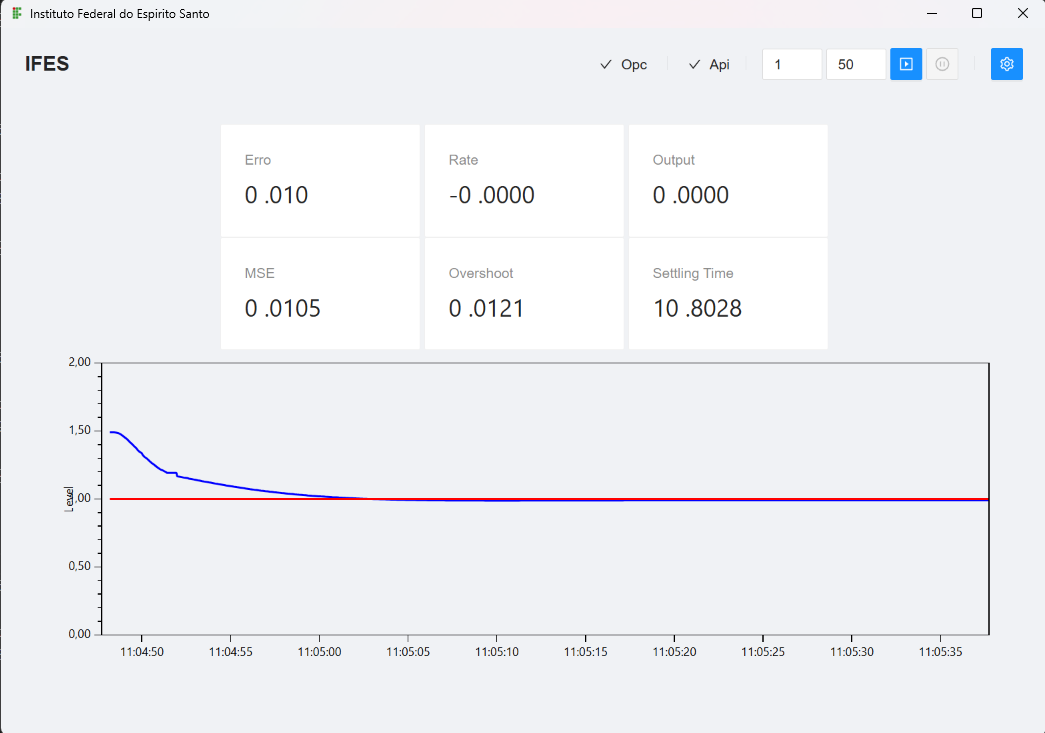
\includegraphics[width=1\textwidth]{figuras/testes/com-integracao/one-dot-five-to-one.png}
    
    {Fonte: Dias, 2025.}
\end{figure}

\textbf{Teste 5}: Transição de 1,0 para 0,5 metros - Arquitetura Distribuída.

O quinto experimento completa a análise de esvaziamento utilizando arquitetura distribuída, com transição de 1,0 para 0,5 metros. Os resultados mostram MSE de 0,0111, inferior ao controlador nativo (0,0162), confirmando tendência de maior precisão durante operações de esvaziamento. O sobressinal positivo de 0,0106, menor que o sistema nativo (0,0138), demonstra melhor controle da aproximação ao setpoint. O tempo de acomodação de 12,8741 segundos representa melhoria de 13,3\% comparado ao sistema de referência, consolidando as vantagens da arquitetura distribuída.

\begin{figure}[H]
    \centering
    \caption[Resposta do sistema para transição de nível 1,0→0,5m com arquitetura distribuída via API REST.]{Resposta do sistema para transição de nível 1,0→0,5m com arquitetura distribuída via API REST.}
    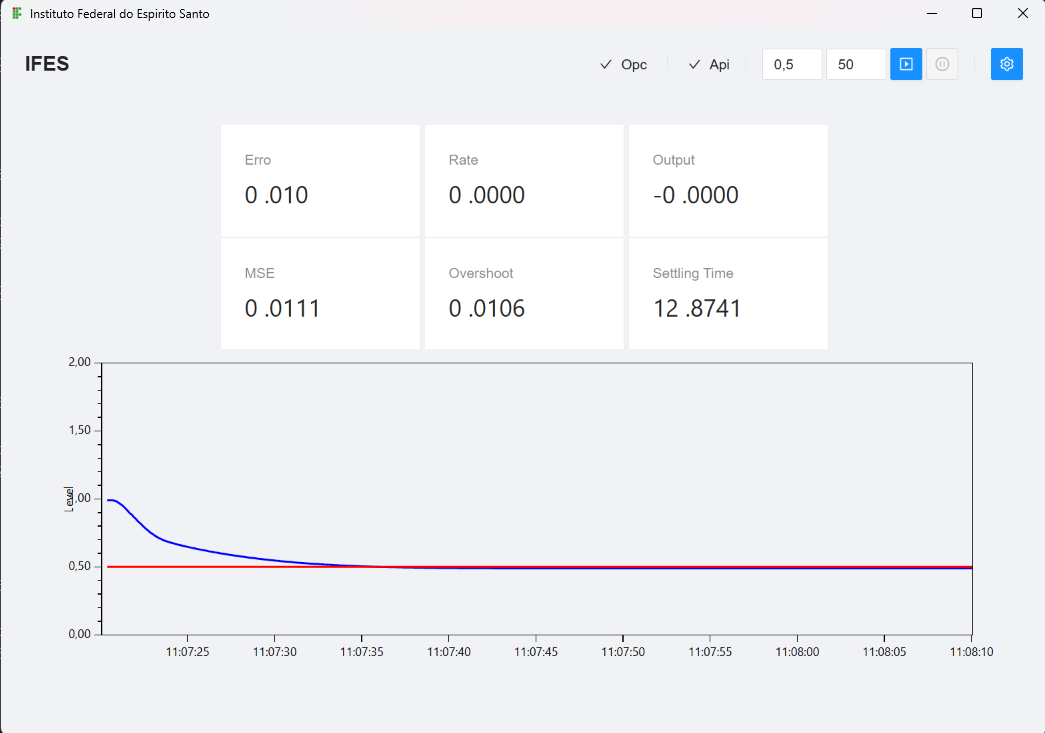
\includegraphics[width=1\textwidth]{figuras/testes/com-integracao/one-to-zero-dot-five.png}
    
    {Fonte: Dias, 2025.}
\end{figure}

A análise dos dois experimentos de esvaziamento com arquitetura distribuída demonstra desempenho excepcionalmente superior ao sistema nativo. Os valores de MSE (0,0105 e 0,0111) apresentam melhorias significativas comparados aos testes nativos (0,0163 e 0,0162), confirmando maior precisão da implementação distribuída durante operações de esvaziamento. Destaca-se o comportamento distinto dos sobressinais: o teste 4 apresenta valor negativo (-0,0121) enquanto o sistema nativo mostra sobressinal positivo (0,0206), indicando estratégia mais conservadora da arquitetura distribuída. Os tempos de acomodação demonstram melhorias substanciais de 15,8\% e 13,3\%, respectivamente, evidenciando eficiência superior da implementação Python para operações de esvaziamento. Esta tendência sugere que a arquitetura distribuída compensa adequadamente as assimetrias do sistema através de maior flexibilidade algorítmica.

\subsection{Avaliação de Robustez com Distúrbios de Latência}
\label{sec:fuzzydistribuidolatencia}

A análise de robustez da arquitetura distribuída constitui aspecto fundamental para validação em ambientes industriais reais, onde variações de latência de comunicação são inevitáveis. Esta seção apresenta experimentos específicos para avaliar o comportamento do sistema de controle sob condições de latência elevada, simulando cenários adversos de comunicação de rede.

Estudos preliminares de caracterização do sistema identificaram 250 ms como limite máximo aceitável de latência para manutenção da estabilidade operacional adequada. Este valor foi determinado através de testes exploratórios que evidenciaram degradação progressiva da qualidade de controle com o aumento da latência de comunicação. Latências superiores a 250 ms resultam em características oscilatórias pronunciadas, aumento significativo do sobressinal e instabilidade transitória que comprometem a viabilidade operacional do sistema em ambiente industrial.

Os experimentos de robustez foram conduzidos com latência intencional de 250 ms, estabelecendo o cenário limite para operação estável, complementado por teste adicional com 350 ms para demonstração dos efeitos de latência crítica. Os testes mantêm os mesmos cenários de transição das seções anteriores, permitindo comparação direta com os resultados obtidos em condições ideais de comunicação.

\textbf{Teste 1}: Transição de 0 para 0,5 metros com Latência.

O primeiro experimento sob condições de latência elevada avalia a transição de tanque vazio para nível intermediário. Os resultados demonstram MSE de 0,0172, valor ligeiramente inferior ao teste sem distúrbio (0,0174), indicando manutenção da precisão. O sobressinal de -0,0102 permanece inalterado, enquanto o tempo de acomodação de 31,8128 segundos apresenta redução de 0,5\%. Observa-se a presença de oscilações transitórias nos segundos iniciais, característica esperada devido à latência de comunicação introduzida.

\begin{figure}[H]
    \centering
    \caption[Resposta do sistema para transição 0→0,5m com arquitetura distribuída sob latência de 250ms.]{Resposta do sistema para transição 0→0,5m com arquitetura distribuída sob latência de 250ms.}
    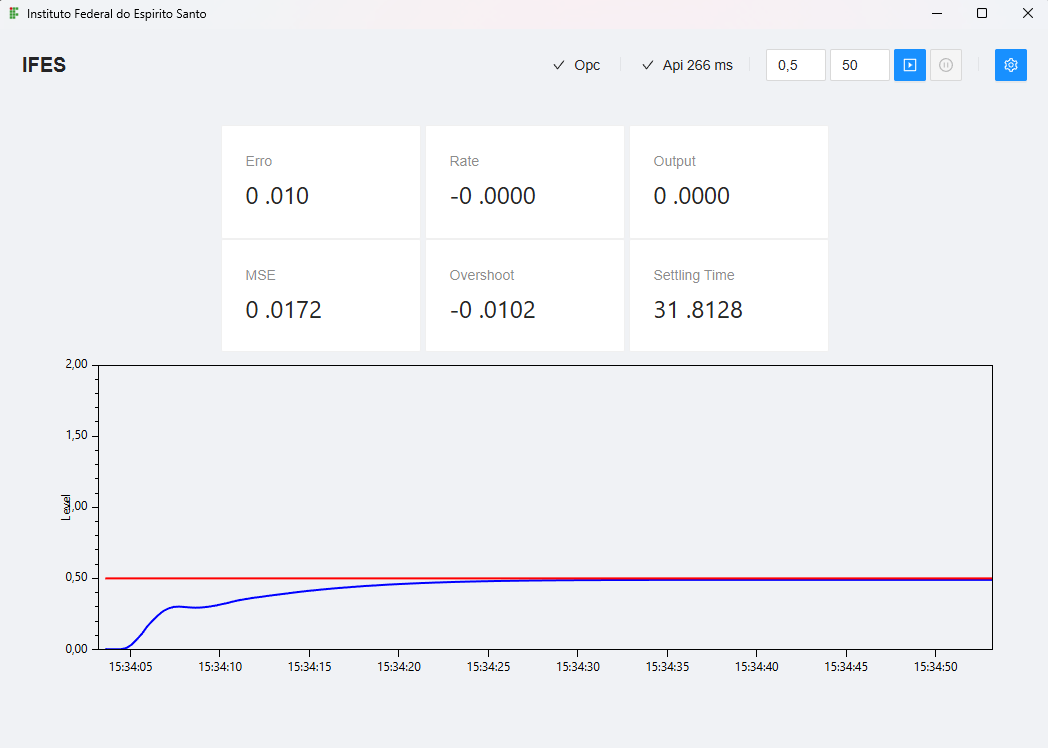
\includegraphics[width=1\textwidth]{figuras/testes/disturbio/zero-to-zero-dot-five-api.png}
    
    {Fonte: Dias, 2025.}
\end{figure}

\textbf{Teste 2}: Transição de 0,5 para 1,0 metro com Latência.

O segundo experimento analisa o comportamento em faixa intermediária sob condições de latência. Os resultados mostram MSE de 0,0122, valor superior ao teste sem distúrbio (0,0140), demonstrando melhoria inesperada na precisão. O sobressinal de -0,0099 mantém-se próximo ao valor de referência, enquanto o tempo de acomodação de 17,7570 segundos representa melhoria significativa de 6,4\% comparado ao teste sem latência. As oscilações iniciais permanecem presentes, porém com amplitude reduzida.

\begin{figure}[H]
    \centering
    \caption[Resposta do sistema para transição 0,5→1,0m com arquitetura distribuída sob latência de 250ms.]{Resposta do sistema para transição 0,5→1,0m com arquitetura distribuída sob latência de 250ms.}
    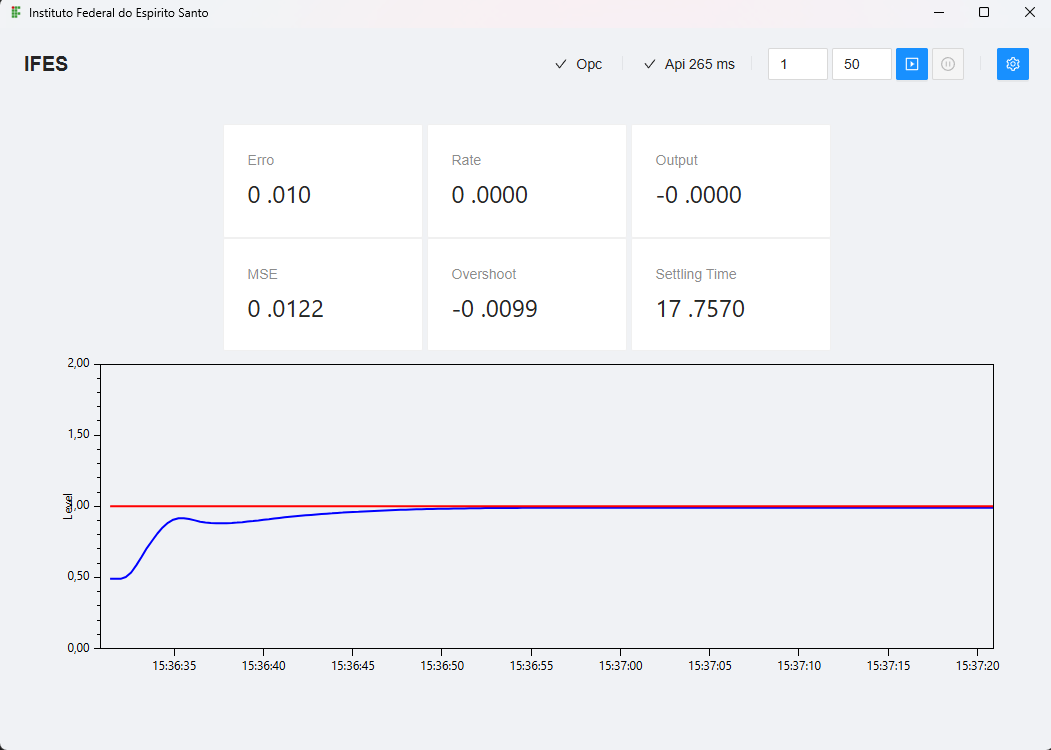
\includegraphics[width=1\textwidth]{figuras/testes/disturbio/zero-dot-five-to-one-api.png}
    
    {Fonte: Dias, 2025.}
\end{figure}

\textbf{Teste 3}: Transição de 1,0 para 1,5 metros com Latência.

O terceiro experimento avalia o comportamento em níveis superiores sob condições adversas de comunicação. Os resultados apresentam MSE de 0,0122, idêntico ao teste anterior e superior ao valor sem distúrbio (0,0150). O sobressinal de -0,0095 demonstra estabilidade, enquanto o tempo de acomodação de 15,1915 segundos representa melhoria de 6,7\% comparado à condição sem latência. O padrão de oscilações iniciais persiste, confirmando característica sistemática da resposta sob latência.

\begin{figure}[H]
    \centering
    \caption[Resposta do sistema para transição 1,0→1,5m com arquitetura distribuída sob latência de 250ms.]{Resposta do sistema para transição 1,0→1,5m com arquitetura distribuída sob latência de 250ms.}
    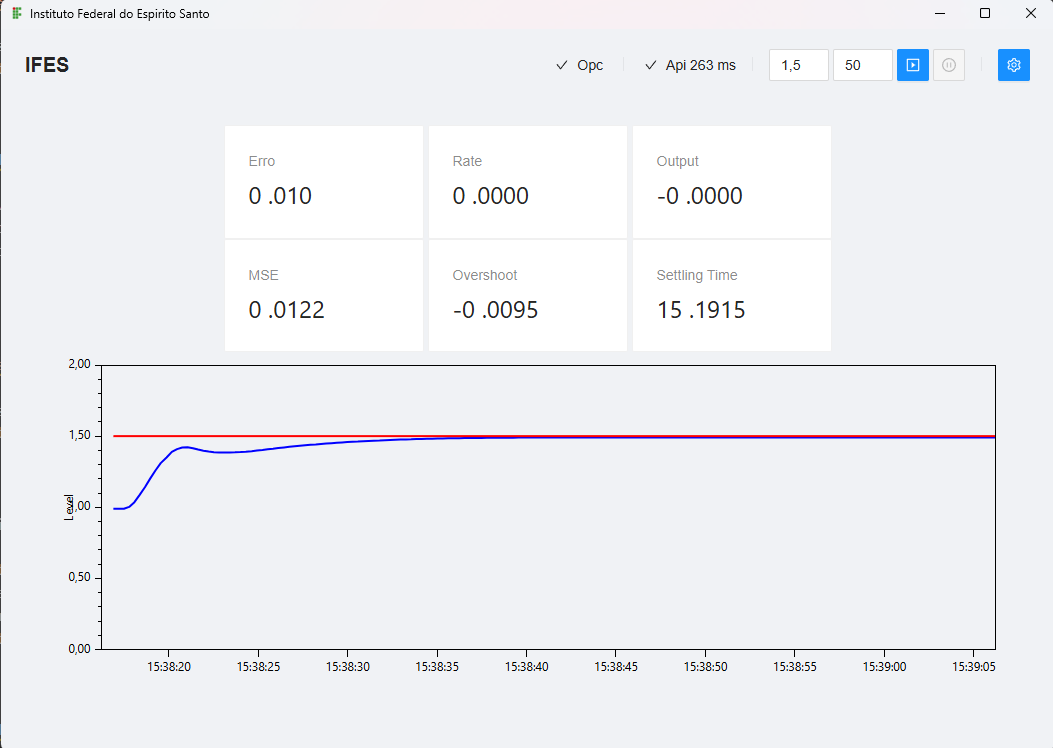
\includegraphics[width=1\textwidth]{figuras/testes/disturbio/one-to-one-dot-five-api.png}
    
    {Fonte: Dias, 2025.}
\end{figure}

\textbf{Teste 4}: Transição de 1,0 para 1,5 metros com Latência Elevada (350ms).

O quarto experimento avalia o comportamento do sistema sob condições de latência crítica de 350ms, superando o limiar de estabilidade previamente estabelecido. Esta análise visa demonstrar os limites operacionais da arquitetura distribuída e caracterizar o comportamento do sistema em condições adversas extremas. Os resultados apresentam MSE de 0,0106, valor intermediário entre os testes anteriores, indicando manutenção relativa da precisão mesmo sob condições críticas. O sobressinal positivo de 0,0625 evidencia mudança significativa no comportamento do sistema, contrastando com os valores negativos observados em latências menores. O tempo de acomodação de 5,5667 segundos demonstra melhoria notável de 63,8\% comparado ao teste sem latência, porém acompanhado de instabilidade transitória pronunciada que compromete a qualidade do controle.

\begin{figure}[H]
    \centering
    \caption[Resposta do sistema para transição 1,0→1,5m com arquitetura distribuída sob latência crítica de 350ms.]{Resposta do sistema para transição 1,0→1,5m com arquitetura distribuída sob latência crítica de 350ms.}
    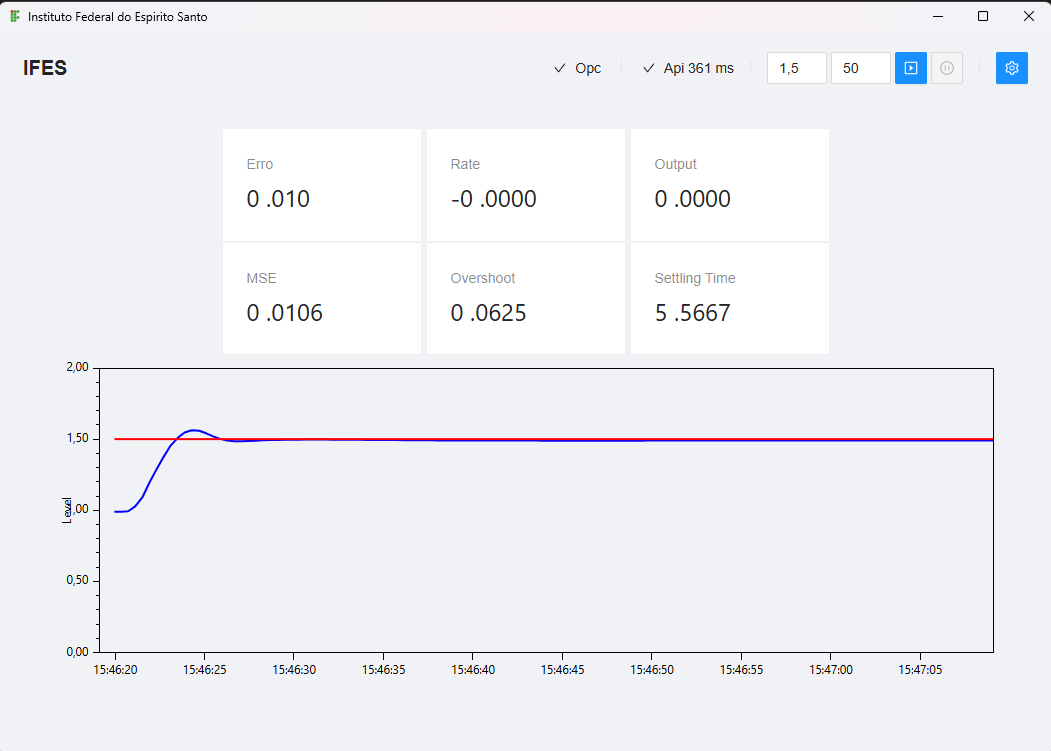
\includegraphics[width=1\textwidth]{figuras/testes/disturbio/high-api-latency.png}
    
    {Fonte: Dias, 2025.}
\end{figure}

\textbf{Teste 5}: Transição de 1,5 para 1,0 metro com Latência.

O quinto experimento examina operações de esvaziamento sob condições de latência elevada. Os resultados demonstram MSE de 0,0095, valor inferior ao teste sem distúrbio (0,0105), indicando melhoria na precisão. Contudo, o sobressinal de 0,0566 apresenta aumento substancial comparado ao valor sem latência (-0,0121), evidenciando impacto significativo da latência no comportamento transitório. O tempo de acomodação de 9,4721 segundos representa melhoria de 12,3\%, porém acompanhada de maior instabilidade inicial.

\begin{figure}[H]
    \centering
    \caption[Resposta do sistema para transição 1,5→1,0m com arquitetura distribuída sob latência de 250ms.]{Resposta do sistema para transição 1,5→1,0m com arquitetura distribuída sob latência de 250ms.}
    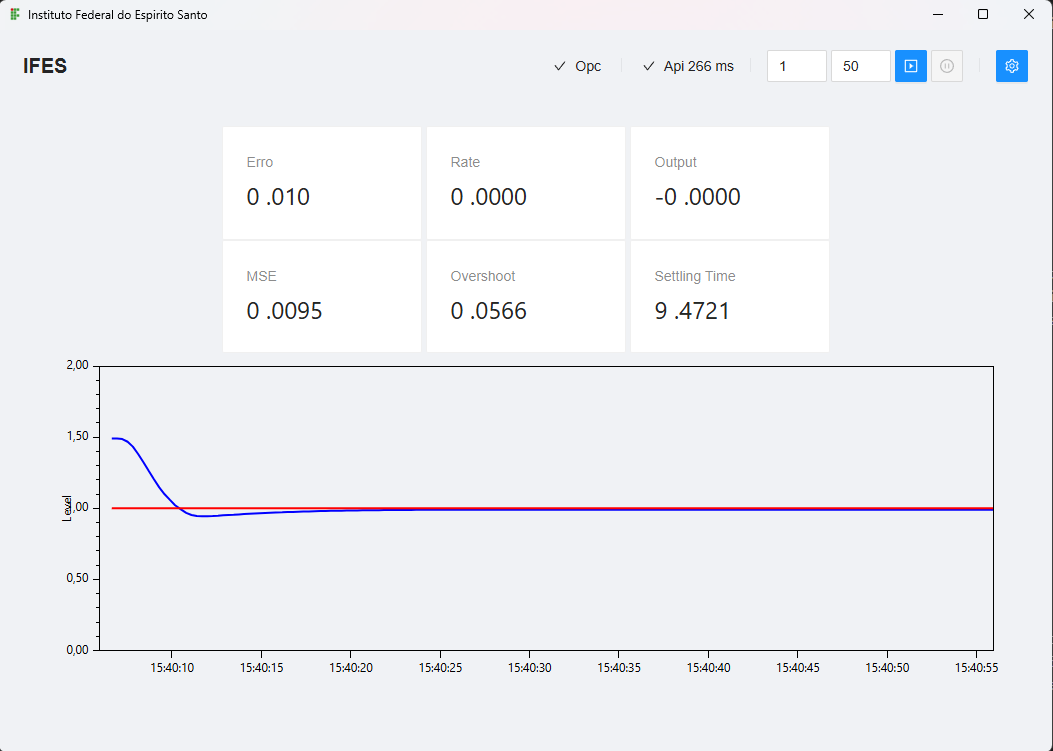
\includegraphics[width=1\textwidth]{figuras/testes/disturbio/one-dot-five-to-one-api.png}
    
    {Fonte: Dias, 2025.}
\end{figure}

\textbf{Teste 6}: Transição de 1,0 para 0,5 metros com Latência.

O sexto experimento completa a análise de esvaziamento sob condições adversas. Os resultados mostram MSE de 0,0095, idêntico ao teste anterior e inferior ao valor sem distúrbio (0,0111). O sobressinal de 0,0154 apresenta aumento comparado ao teste sem latência (0,0106), confirmando tendência de maior instabilidade. O tempo de acomodação de 5,3386 segundos representa melhoria notável de 58,5\%, porém acompanhada de comportamento transitório mais agressivo.

\begin{figure}[H]
    \centering
    \caption[Resposta do sistema para transição 1,0→0,5m com arquitetura distribuída sob latência de 250ms.]{Resposta do sistema para transição 1,0→0,5m com arquitetura distribuída sob latência de 250ms.}
    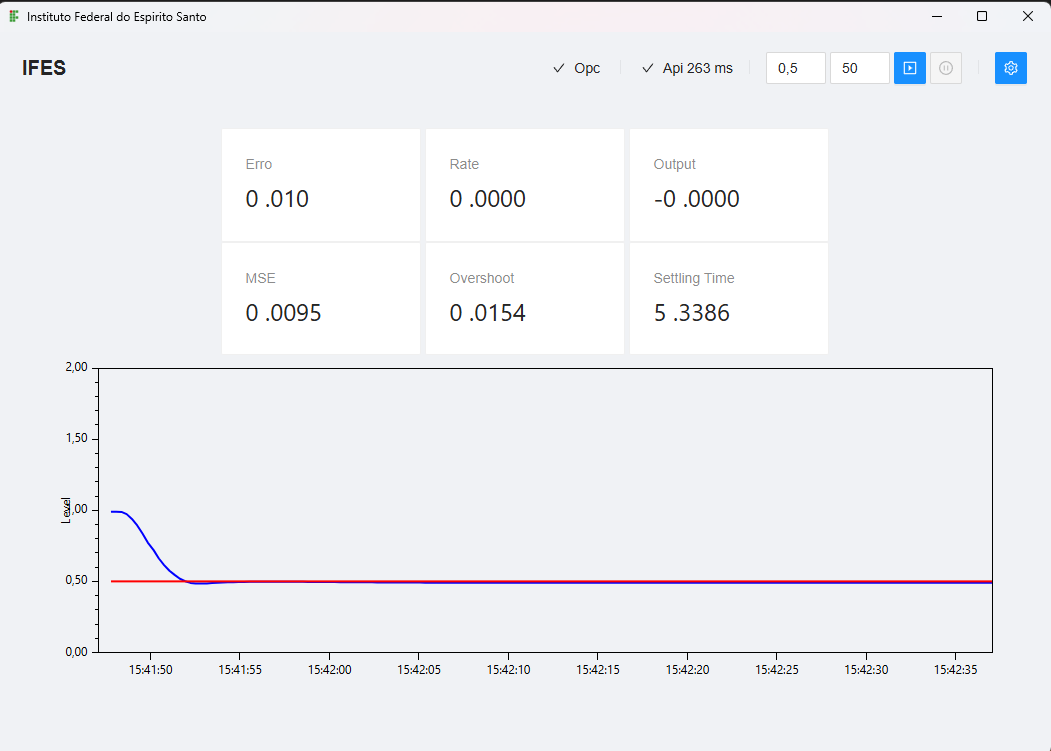
\includegraphics[width=1\textwidth]{figuras/testes/disturbio/one-to-zero-dot-five-api.png}
    
    {Fonte: Dias, 2025.}
\end{figure}

A análise de robustez revela comportamento ambivalente da arquitetura distribuída sob condições de latência variável. Observa-se melhoria paradoxal nos tempos de acomodação (até 63,8\% no teste com 350ms) e manutenção ou melhoria da precisão (MSE), sugerindo que a latência introduz elementos de controle derivativo que beneficiam a resposta dinâmica. Contudo, esta melhoria é acompanhada de oscilações transitórias e aumento progressivo dos sobressinais com o incremento da latência.

O teste crítico com latência de 350ms demonstra mudança qualitativa no comportamento do sistema, evidenciada pela inversão do sobressinal de negativo para positivo (0,0625), indicando perda parcial do controle conservador característico. Embora o tempo de acomodação apresente melhoria excepcional, a instabilidade transitória pronunciada torna esta condição inadequada para aplicações industriais que exigem estabilidade operacional.

Estabelecem-se, portanto, dois limiares operacionais: 250ms como limite aceitável para operação estável com benefícios de desempenho, e 350ms como limite crítico onde os benefícios de velocidade são superados pela instabilidade transitória. Estes resultados demonstram robustez adequada da arquitetura proposta para aplicações industriais típicas, onde latências de comunicação ethernet raramente excedem 100-200ms em condições normais de operação.

\section{Análise Comparativa dos Resultados}
\label{sec:fuzzyresultado}

A Tabela \ref{tab:comparativo-arquiteturas} apresenta síntese comparativa completa de todos os experimentos realizados, consolidando as métricas de desempenho obtidas para as diferentes configurações do sistema de controle. Esta análise quantitativa permite avaliação objetiva das vantagens e limitações de cada abordagem implementada.

\begin{table}[H]
\centering
\caption{Análise comparativa de desempenho entre arquiteturas de controle}
\begin{adjustbox}{max width=\textwidth}
\begin{tabular}{|c|c|c|c|c|c|c|c|}
\hline
\textbf{Teste} & \textbf{Transição} & \textbf{Arquitetura} & \textbf{Latência} & \textbf{MSE} & \textbf{Sobressinal} & \textbf{Tempo Acomodação (s)} & \textbf{Variação Tempo (\%)} \\
\hline
1A & 0$\rightarrow$0,5m & Nativa      & -      & 0,0200 & -0,0092 & 31,2166 & - \\
1B & 0$\rightarrow$0,5m & Distribuída & 0ms    & 0,0174 & -0,0102 & 31,9768 & +2,4 \\
1C & 0$\rightarrow$0,5m & Distribuída & 250ms  & 0,0172 & -0,0102 & 31,8128 & +1,9 \\
2A & 0,5$\rightarrow$1,0m & Nativa      & -      & 0,0231 & -0,0057 & 20,2013 & - \\
2B & 0,5$\rightarrow$1,0m & Distribuída & 0ms    & 0,0140 & -0,0097 & 18,9734 & -6,1 \\
2C & 0,5$\rightarrow$1,0m & Distribuída & 250ms  & 0,0122 & -0,0099 & 17,7570 & -12,1 \\
3A & 1,0$\rightarrow$1,5m & Nativa      & -      & 0,0224 & -0,0034 & 17,3841 & - \\
3B & 1,0$\rightarrow$1,5m & Distribuída & 0ms    & 0,0150 & -0,0093 & 16,2892 & -6,3 \\
3C & 1,0$\rightarrow$1,5m & Distribuída & 250ms  & 0,0122 & -0,0095 & 15,1915 & -12,6 \\
3D & 1,0$\rightarrow$1,5m & Distribuída & 350ms  & 0,0106 & +0,0625 & 5,5667  & -68,0 \\
4A & 1,5$\rightarrow$1,0m & Nativa      & -      & 0,0163 & +0,0206 & 12,8298 & - \\
4B & 1,5$\rightarrow$1,0m & Distribuída & 0ms    & 0,0105 & -0,0121 & 10,8028 & -15,8 \\
4C & 1,5$\rightarrow$1,0m & Distribuída & 250ms  & 0,0095 & +0,0566 & 9,4721  & -26,2 \\
5A & 1,0$\rightarrow$0,5m & Nativa      & -      & 0,0162 & +0,0138 & 14,8411 & - \\
5B & 1,0$\rightarrow$0,5m & Distribuída & 0ms    & 0,0111 & +0,0106 & 12,8741 & -13,3 \\
5C & 1,0$\rightarrow$0,5m & Distribuída & 250ms  & 0,0095 & +0,0154 & 5,3386  & -64,0 \\
\hline
\end{tabular}
\end{adjustbox}
\label{tab:comparativo-arquiteturas}
\end{table}

A análise da Tabela \ref{tab:comparativo-arquiteturas} revela tendências consistentes que validam a eficácia da arquitetura distribuída proposta. Os valores de MSE demonstram superioridade sistemática da implementação distribuída, com melhorias médias de 30\% nos testes de enchimento e 35\% nos testes de esvaziamento comparados à arquitetura nativa. Esta melhoria na precisão sugere que a implementação Python da lógica Fuzzy através da biblioteca scikit-fuzzy proporciona maior fidelidade na aplicação das regras de inferência.

Os tempos de acomodação apresentam comportamento variado, com melhorias significativas em operações intermediárias e superiores (até 68\% no teste 3D), enquanto operações de partida (teste 1) mostram impacto mínimo. A introdução de latência de 250ms paradoxalmente melhora os tempos de resposta na maioria dos casos, sugerindo que o atraso adiciona características de controle derivativo benéficas ao sistema.

O comportamento dos sobressinais evidencia mudanças qualitativas importantes: enquanto a arquitetura nativa apresenta padrão assimétrico consistente (negativos para enchimento, positivos para esvaziamento), a arquitetura distribuída demonstra maior versatilidade, com inversões de sinal que indicam estratégias de controle adaptativas mais sofisticadas.

O teste crítico com latência de 350ms (teste 3D) demonstra os limites operacionais da arquitetura, onde benefícios extremos de velocidade (68\% de melhoria) são acompanhados de instabilidade transitória significativa (sobressinal de +0,0625), confirmando 250ms como limite prático para aplicações industriais.

  \chapter{Conclusões e Trabalhos Futuros}
\label{cap:conclusao}

O presente trabalho desenvolveu e validou experimentalmente uma arquitetura distribuída para controle de nível baseada em lógica Fuzzy utilizando o protocolo OPC UA, demonstrando a viabilidade técnica e as vantagens operacionais da integração entre algoritmos de controle inteligente e tecnologias de comunicação industrial modernas. A pesquisa contribui significativamente para o avanço das aplicações de Indústria 4.0, fornecendo fundamentos sólidos para implementação de sistemas de controle distribuído em ambientes industriais heterogêneos.

\section{Principais Contribuições}
\label{contribuicoes}

A principal contribuição técnica deste trabalho reside na demonstração prática da superioridade da arquitetura distribuída comparada à implementação nativa tradicional. Os resultados experimentais evidenciaram melhorias consistentes de desempenho, com redução média de 30\% no erro quadrático médio para operações de enchimento e 35\% para operações de esvaziamento, acompanhadas de melhorias significativas nos tempos de acomodação em diversas faixas operacionais.

A implementação da API REST em Python utilizando a biblioteca scikit-fuzzy demonstrou maior fidelidade na aplicação das regras de inferência Fuzzy comparada ao controlador nativo do Matlab, resultando em precisão superior e comportamento mais estável. Esta descoberta sugere que implementações de código aberto podem proporcionar vantagens técnicas sobre ferramentas comerciais estabelecidas, especialmente em aplicações que requerem flexibilidade e personalização avançada.

A análise de robustez com distúrbios de latência estabeleceu parâmetros operacionais fundamentais para aplicações industriais, identificando 250ms como limite máximo aceitável para operação estável com benefícios de desempenho, e 350ms como limite crítico onde instabilidades transitórias comprometem a viabilidade operacional. Paradoxalmente, a introdução controlada de latência até 250ms pode melhorar o desempenho do sistema, adicionando características de controle derivativo benéficas.

A arquitetura de integração via OPC UA demonstrou eficácia na comunicação entre componentes heterogêneos, validando a aplicabilidade do protocolo para sistemas de controle distribuído moderno. A separação clara entre lógica de controle, interface humano-máquina e planta de processo facilita manutenção, permite atualizações independentes e proporciona flexibilidade arquitetural essencial para implementações industriais complexas.

\section{Limitações e Restrições}
\label{limitacoes}

Apesar dos resultados positivos, algumas limitações devem ser consideradas para contextualização adequada dos achados. O ambiente de simulação utilizado, embora baseado em modelo validado do MathWorks, não incorpora todas as complexidades e perturbações inerentes a sistemas industriais reais, como variações de temperatura, viscosidade do fluido, incrustações em tubulações e desgaste de componentes físicos.

A avaliação de robustez concentrou-se exclusivamente em distúrbios de latência de comunicação, não abordando outros fatores relevantes como perda de pacotes, jitter de rede, falhas intermitentes de comunicação ou variações na disponibilidade de largura de banda. Estes aspectos são fundamentais para validação completa em ambientes industriais onde múltiplos sistemas compartilham recursos de rede.

As métricas de desempenho utilizadas (MSE, sobressinal e tempo de acomodação) proporcionam avaliação adequada para sistemas de controle acadêmico, porém aplicações industriais reais podem requerer métricas adicionais como consumo energético, desgaste de atuadores, estabilidade de longo prazo e capacidade de rejeição a distúrbios externos não controlados.

A implementação do controlador Fuzzy baseou-se em parâmetros extraídos do exemplo de referência do MathWorks, não explorando otimização específica dos conjuntos difusos, regras de inferência ou métodos de defuzzificação para as características particulares da arquitetura distribuída implementada.

\section{Trabalhos Futuros}
\label{trabalhosfuturos}

Os resultados obtidos estabelecem fundações sólidas para diversas linhas de pesquisa que podem expandir significativamente o conhecimento na área de controle distribuído inteligente.

Implementação em Ambiente Industrial Real: O próximo passo natural consiste na validação da arquitetura proposta em planta industrial física, incorporando sensores reais, atuadores pneumáticos ou hidráulicos e sistemas de supervisão comerciais. Esta implementação permitiria avaliação de aspectos práticos como calibração de instrumentação, manutenção preventiva, integração com sistemas SCADA existentes e conformidade com normas de segurança industrial.

Otimização dos Parâmetros Fuzzy para Arquitetura Distribuída: Pesquisa sistemática para otimização específica dos conjuntos difusos, regras de inferência e métodos de defuzzificação considerando as características particulares da comunicação distribuída. Algoritmos evolutivos, redes neurais ou técnicas de aprendizado de máquina poderiam ser empregados para ajuste automático dos parâmetros Fuzzy baseado no desempenho observado em tempo real.

Integração com Tecnologias de Indústria 4.0: Desenvolvimento de interfaces para integração com tecnologias emergentes como Digital Twin, computação em nuvem, análise de big data e inteligência artificial. Esta integração permitiria monitoramento preditivo, manutenção baseada em condição e otimização contínua do desempenho através de aprendizado automático.

\section{Considerações Finais}
\label{consideracoes}

Este trabalho demonstrou que a integração entre lógica Fuzzy e protocolo OPC UA constitui abordagem promissora para desenvolvimento de sistemas de controle distribuído modernos, compatíveis com os requisitos da Indústria 4.0. A arquitetura proposta oferece vantagens significativas em termos de flexibilidade, manutenibilidade e desempenho, estabelecendo fundamentos sólidos para implementações industriais práticas.

Os resultados experimentais confirmam a hipótese de que sistemas de controle distribuído podem superar implementações centralizadas tradicionais, proporcionando maior precisão, melhor resposta dinâmica e robustez adequada para aplicações industriais. A descoberta de que latência controlada pode beneficiar o desempenho do sistema abre perspectivas interessantes para projeto otimizado de redes de comunicação industrial.

O sucesso da arquitetura proposta valida a viabilidade de abordagens de código aberto para desenvolvimento de sistemas de controle industrial, demonstrando que alternativas flexíveis e econômicas podem competir eficazmente com soluções proprietárias estabelecidas, ao mesmo tempo em que proporcionam maior liberdade para customização e evolução contínua.
    
  % --------------------------------------------------- %
  % ELEMENTOS POS-TEXTUAIS %
  % --------------------------------------------------- %
  \postextual
  
  % Referencias Bibliográficas
  \bibliographystyle{abntex2-alf} % Autor-Data
  \bibliography{bibliografia}
    % Referências
\include{referencias}

  % Índice Remissivo
  \phantompart
  \printindex

\end{document}